% $Id: template.tex 11 2007-04-03 22:25:53Z jpeltier $

% \documentclass{vgtc}                          % final (conference style)
\documentclass[review]{vgtc}                 % review
%\documentclass[widereview]{vgtc}             % wide-spaced review
%\documentclass[preprint]{vgtc}               % preprint
%\documentclass[electronic]{vgtc}             % electronic version

%% Uncomment one of the lines above depending on where your paper is
%% in the conference process. ``review'' and ``widereview'' are for review
%% submission, ``preprint'' is for pre-publication, and the final version
%% doesn't use a specific qualifier. Further, ``electronic'' includes
%% hyperreferences for more convenient online viewing.

%% Please use one of the ``review'' options in combination with the
%% assigned online id (see below) ONLY if your paper uses a double blind
%% review process. Some conferences, like IEEE Vis and InfoVis, have NOT
%% in the past.

%% Figures should be in CMYK or Grey scale format, otherwise, colour 
%% shifting may occur during the printing process.

%% These few lines make a distinction between latex and pdflatex calls and they
%% bring in essential packages for graphics and font handling.
%% Note that due to the \DeclareGraphicsExtensions{} call it is no longer necessary
%% to provide the the path and extension of a graphics file:
%% \includegraphics{diamondrule} is completely sufficient.
%%
\ifpdf%                                % if we use pdflatex
  \pdfoutput=1\relax                   % create PDFs from pdfLaTeX
  \pdfcompresslevel=9                  % PDF Compression
  \pdfoptionpdfminorversion=7          % create PDF 1.7
  \ExecuteOptions{pdftex}
  \usepackage{graphicx}                % allow us to embed graphics files
  \DeclareGraphicsExtensions{.pdf,.png,.jpg,.jpeg} % for pdflatex we expect .pdf, .png, or .jpg files
\else%                                 % else we use pure latex
  \ExecuteOptions{dvips}
  \usepackage{graphicx}                % allow us to embed graphics files
  \DeclareGraphicsExtensions{.eps}     % for pure latex we expect eps files
\fi%

%% it is recomended to use ``\autoref{sec:bla}'' instead of ``Fig.~\ref{sec:bla}''
\graphicspath{{figures/}{pictures/}{images/}{./}} % where to search for the images

\usepackage{microtype}                 % use micro-typography (slightly more compact, better to read)
\PassOptionsToPackage{warn}{textcomp}  % to address font issues with \textrightarrow
\usepackage{textcomp}                  % use better special symbols
\usepackage{mathptmx}                  % use matching math font
\usepackage{times}                     % we use Times as the main font
\renewcommand*\ttdefault{txtt}         % a nicer typewriter font
\usepackage{cite}                      % needed to automatically sort the references
\usepackage{tabu}                      % only used for the table example
\usepackage{booktabs}                  % only used for the table example
%% We encourage the use of mathptmx for consistent usage of times font
%% throughout the proceedings. However, if you encounter conflicts
%% with other math-related packages, you may want to disable it.


%% If you are submitting a paper to a conference for review with a double
%% blind reviewing process, please replace the value ``0'' below with your
%% OnlineID. Otherwise, you may safely leave it at ``0''.
\onlineid{0}

%% declare the category of your paper, only shown in review mode
\vgtccategory{Research}

%% allow for this line if you want the electronic option to work properly
\vgtcinsertpkg

%% In preprint mode you may define your own headline.
%\preprinttext{To appear in an IEEE VGTC sponsored conference.}

%% Paper title.

\title{User Evaluation of Group-in-a-box Variants}

%% This is how authors are specified in the conference style

%% Author and Affiliation (single author).
%%\author{Roy G. Biv\thanks{e-mail: roy.g.biv@aol.com}}
%%\affiliation{\scriptsize Allied Widgets Research}

%% Author and Affiliation (multiple authors with single affiliations).
%%\author{Roy G. Biv\thanks{e-mail: roy.g.biv@aol.com} %
%%\and Ed Grimley\thanks{e-mail:ed.grimley@aol.com} %
%%\and Martha Stewart\thanks{e-mail:martha.stewart@marthastewart.com}}
%%\affiliation{\scriptsize Martha Stewart Enterprises \\ Microsoft Research}

%% Author and Affiliation (multiple authors with multiple affiliations)
\author{Nozomi Aoyama\thanks{e-mail: aoyama.nozomi.37x@st.kyoto-u.ac.jp}\\ %
        \scriptsize Kyoto University %
\and Yosuke Onoue\thanks{e-mail: onoue.yousuke@nihon-u.ac.jp}\\ %
     \scriptsize Nihon University %
\and Yuki Ueno\thanks{e-mail: ueno.yuki.78x@st.kyoto-u.ac.jp}\\ %
     % \parbox{1.4in}{
     \scriptsize \centering Kyoto University
\and Hiroaki Natsukawa\thanks{e-mail: natsukawa.hiroaki.3u@kyoto-u.ac.jp}\\ %
     \scriptsize Kyoto University
\and Koji Koyamada\thanks{e-mail: koyamada.koji.3w@kyoto-u.ac.jp}\\ %
     \scriptsize Kyoto University}

%% A teaser figure can be included as follows, but is not recommended since
%% the space is now taken up by a full width abstract.
%\teaser{
%  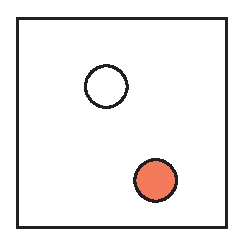
\includegraphics[width=1.5in]{sample.eps}
%  \caption{Lookit! Lookit!}
%}

%% Abstract section.
\abstract{
Group in a box (GIB) is a graph-drawing method designed for visualizing the group structure of graphs.
GIB allows group sizes and both the inter- and intra-group structures to be viewed simultaneously.
Several GIB variants have been proposed to realize each design
goal.
However, their advantages and disadvantages have not been studied from the perspective of human cognition.
Therefore, we conducted a user evaluation, which included eye-tracking analysis, on four GIB variants, namely ST-GIB, CD-GIB, FD-GIB and TR-GIB.
As a result, we found some trade-offs among the methods for the type of user task, and we revealed the superiority of FD-GIB and TR-GIB.
Although ST-GIB did not give a bad result, it was inferior in terms of the link readability.
The eye-tracking analysis provided some clues as to why these results were generated and which elements in a visualization affected the experimental results.
We also provide a website where the four GIB layouts are available.
This study will encourage effective use of GIB to promote analysis of network diagrams such as social networks or web graphs.
} % end of abstract

%% ACM Computing Classification System (CCS). 
%% See <http://www.acm.org/about/class> for details.
%% We recommend the 2012 system <http://www.acm.org/about/class/class/2012>
%% For the 2012 system use the ``\CCScatTwelve'' which command takes four arguments.
%% The 1998 system <http://www.acm.org/about/class/class/2012> is still possible
%% For the 1998 system use the ``\CCScat'' which command takes four arguments.
%% In both cases the last two arguments (1998) or last three (2012) can be empty.

\CCScatlist{
  \CCScatTwelve{Human-centered computing}{Visu\-al\-iza\-tion}{Visu\-al\-iza\-tion techniques}{Graph drawings};
  \CCScatTwelve{Human-centered computing}{Visu\-al\-iza\-tion}{Visualization design and evaluation methods}{}
}

%\CCScatlist{
  %\CCScat{H.5.2}{User Interfaces}{User Interfaces}{Graphical user interfaces (GUI)}{};
  %\CCScat{H.5.m}{Information Interfaces and Presentation}{Miscellaneous}{}{}
%}

%% Copyright space is enabled by default as required by guidelines.
%% It is disabled by the 'review' option or via the following command:
% \nocopyrightspace

%%%%%%%%%%%%%%%%%%%%%%%%%%%%%%%%%%%%%%%%%%%%%%%%%%%%%%%%%%%%%%%%
%%%%%%%%%%%%%%%%%%%%%% START OF THE PAPER %%%%%%%%%%%%%%%%%%%%%%
%%%%%%%%%%%%%%%%%%%%%%%%%%%%%%%%%%%%%%%%%%%%%%%%%%%%%%%%%%%%%%%%%

\begin{document}

%% The ``\maketitle'' command must be the first command after the
%% ``\begin{document}'' command. It prepares and prints the title block.

%% the only exception to this rule is the \firstsection command
\firstsection{Introduction}

\maketitle

%% \section{Introduction} %for journal use above \firstsection{..} instead
In the field of graph drawing, numerous methods have been proposed, each aiming at a different visualization goal.
Some methods are designed for the analysis of real-world graph data such as social networks and web graphs.
They are often characterized as being so-called complex networks~\cite{Newman:2010:NI:1809753}, a feature of which is their community structure~\cite{girvan2002community,newman2004detecting}.
A network with a community structure contains groups and nodes which belong to the groups.
Additionally, certain groups in this kind of data have dense within-group edges and sparse between-group edges.
For example, consider Twitter network data, which has users as nodes and edges connecting couples of users representing one replies to or mentions the other.
Users can be divided into some groups in such a network using the topology of the graph or its feature.
When a network becomes larger and has higher density, it can be more challenging for an observer to understand the network’s data because of the high number of nodes, edges, and groups, resulting in a visual clutter.
To analyze real-world data, an effective visualization technique for understanding group structure of a network is essential.

There are various methods to group related nodes in a network based on a feature of that such as the topology, some attributes the nodes have, or the combination of them~\cite{clauset2004finding,wakita2007finding,lloyd1982least,navlakha2009finding}.
A topological method generates groups so that the relationships among nodes in a single group are stronger than those between nodes in different groups.
The latter method takes some common attributes of the nodes. For example, in the case of a Twitter network, there are users' geographical locations, religions, and interests.
General methods to illustrate these groups visually discriminate them by the color or shape of nodes, which does not make groups easy to understand in a large network.

Group in a box (GIB) is a graph-drawing method designed for a network in which a node belongs to a group and visualizing the group structures in graphs.
GIB arranges all nodes in a group into a box with an area proportional to the number of nodes in the group so that each group can be visualized separately.
Using a GIB layout enables simultaneous visualization of group structures, group relationships, inter-group relationships, and the sizes of the groups in a graph.
Specifically, it is expected that placing groups in individual boxes aids in the understanding of the information within a group.
There are several variants of GIB layout~\cite{rodrigues2011group,chaturvedi2014group,onoue2017optimal}, and each of them has a different original purpose.
Although some computational experiments~\cite{chaturvedi2014group,onoue2017optimal} have evaluated these GIB variants, to the best of our knowledge, no evaluations have been made through user experiments.
Some network measures are used in the abovementioned computational experiments (e.g., the number of edge crossings) known to affect the readability of a graph drawing~\cite{468391,purchase1997aesthetic,purchase1998performance,purchase2002empirical}, but other elements related to readability in GIB visualizations make user experiments important.

Therefore, we aim to ascertain which GIB variant is the most effective.
We report on the evaluations of four GIB variants, namely ST-GIB, CD-GIB, FD-GIB, and TR-GIB, with four types of user task. The tasks are designed based on the studies by Vehlow et al.
\cite{Vehlow2017VisualizingGS} and Saket et al.~\cite{saket2014group} to view each layout's features from various perspectives.
We measure the accuracy and completion time for each task.
We also collect eye-tracking data from participants.

Eye-tracking is a technique used to record gaze data and is often used in user experiments in the field of visualization and human-computer interaction.
It is useful for analyzing tasks in this case because the gaze data of participants can give us some insights into why each layout affects the results~\cite{andrienko2012visual,duchowski2007eye,kurzhals2014evaluating}.
Along with the accuracy and completion time of tasks, we also analyze eye-tracking data to reveal the differences between layout.
Specifically, we focus on finding out which elements in a layout make it easy or difficult to solve tasks.

One of our main contributions is the evaluation of 4 GIB layouts and to determine the best GIB.
We assume that each GIB has advantage and disadvantage, so we aim to evaluate these GIB variants with 4 tasks and verify which is significantly superior in each task.
We also provide some evidence to support our results using the eye tracking data with an aim to clarify which elements in a visualization affect the results.
In addition, we make these 4 GIB layouts available to the public. Our website provides GIB images~\cite{gibweb}, as well as further analysis of the network. This can help researchers in analyzing their network data and possibly lead them to new findings.

\begin{figure*}[t]
  \begin{center}
    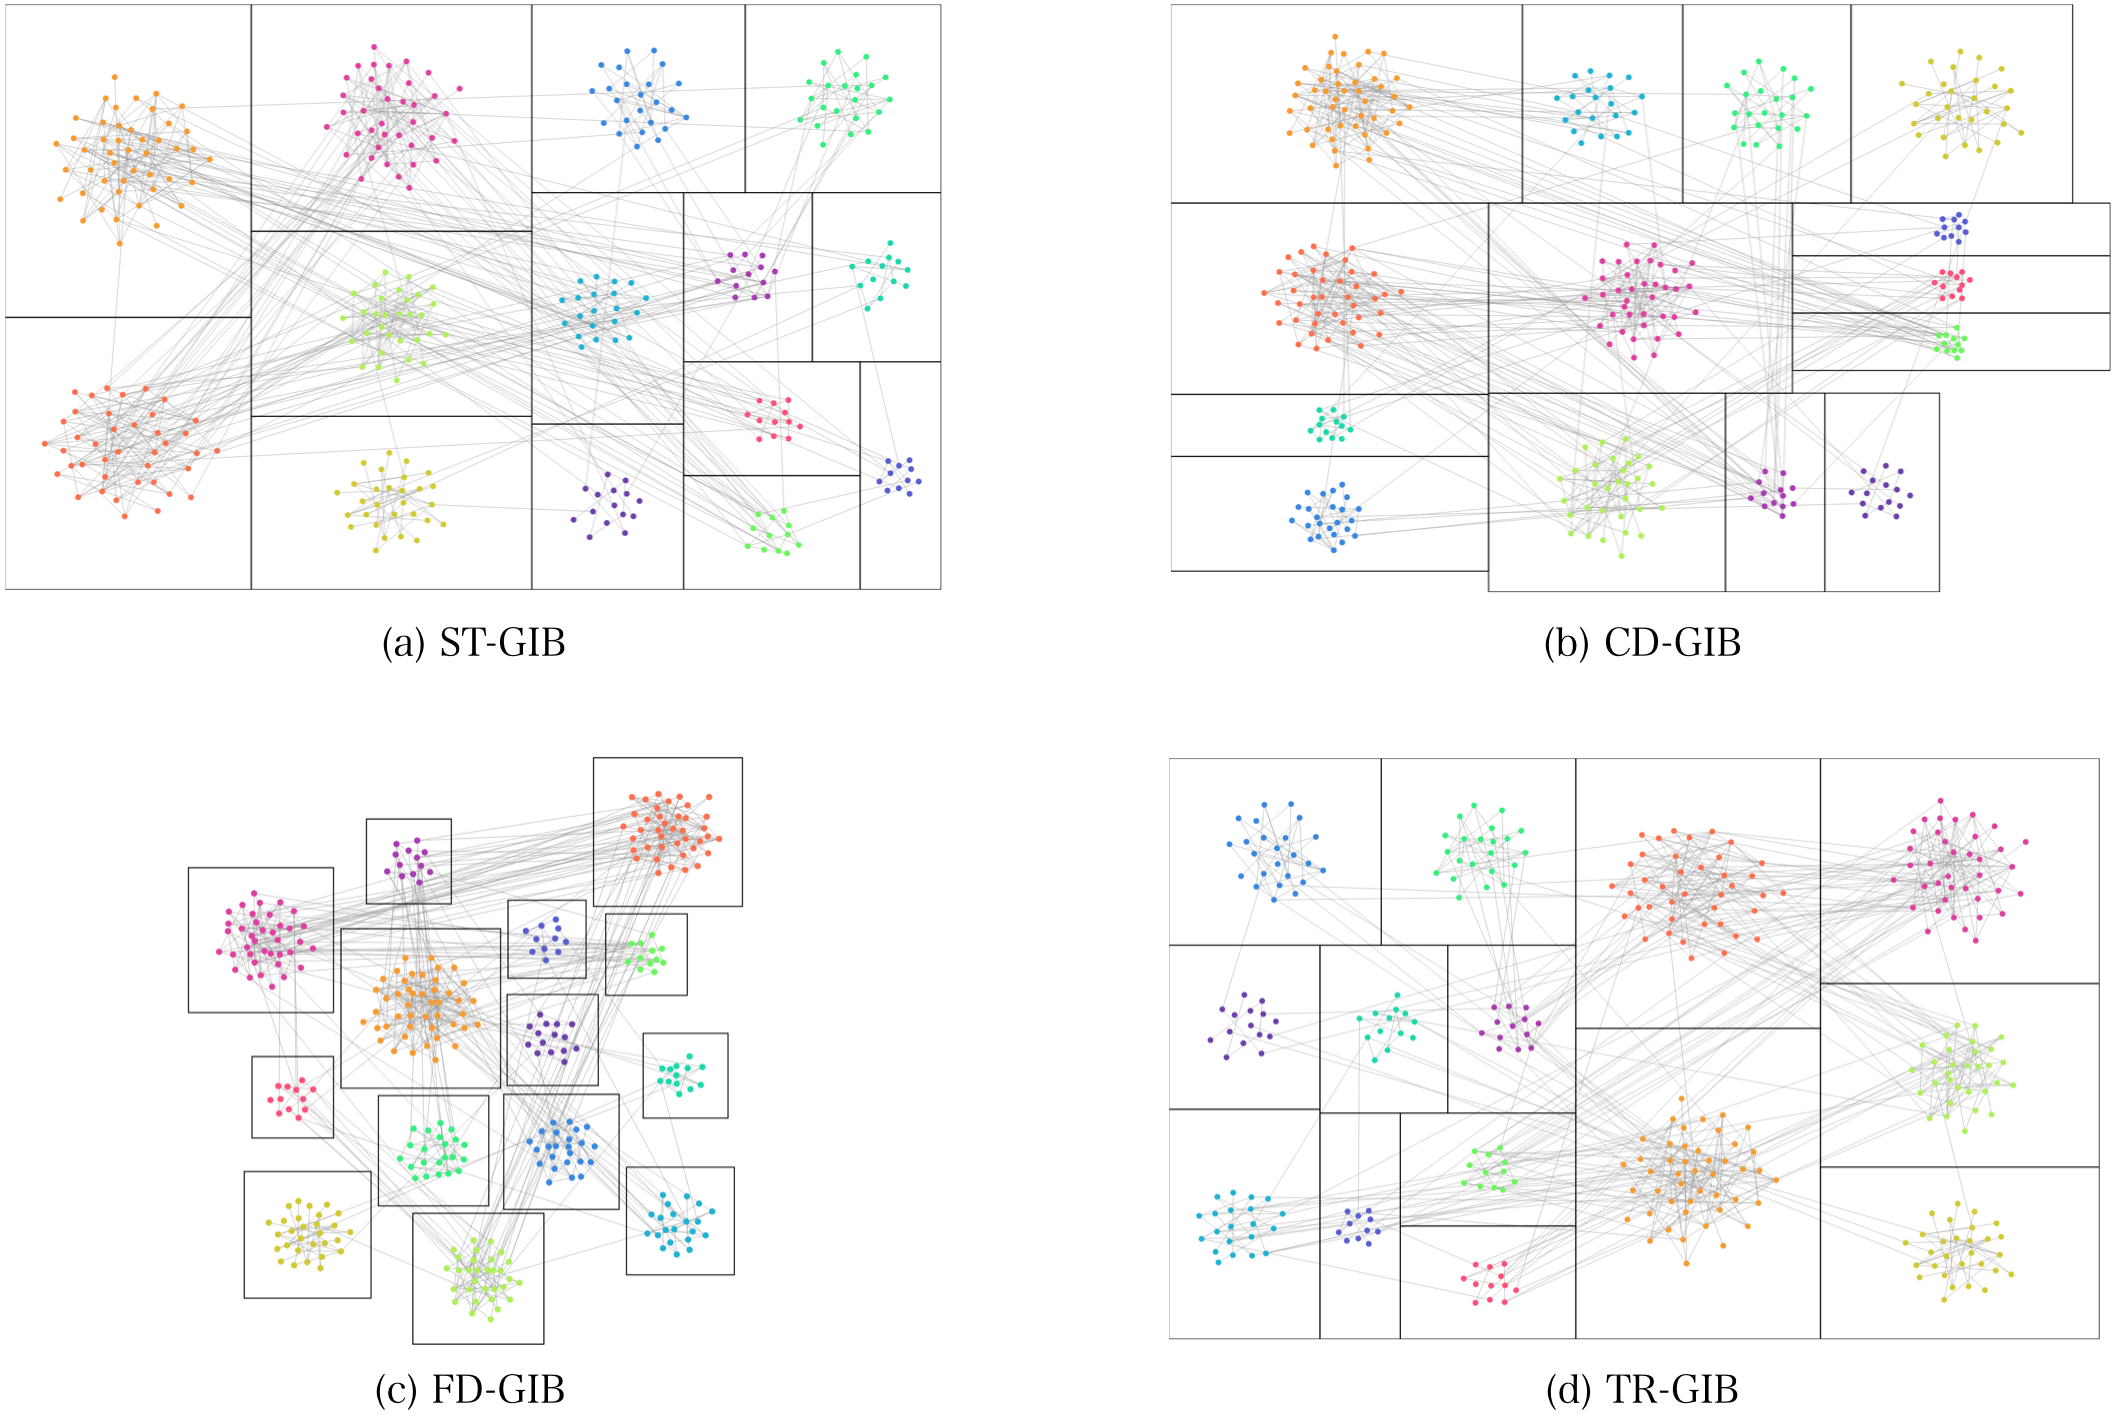
\includegraphics[width=1\textwidth]{pictures/examples.png}
    \caption{Examples of group-in-a-box (GIB) layouts. Four GIB layout look different but the original data is the same. (a)~ST-GIB is based on treemapping. (b)~CD-GIB considers the information of links connecting groups. (c)~FD-GIB arranges the boxes with force-directed layout. (d)~TR-GIB is what we reordered the rectangles in ST-GIB to minimize the group proximity.}
    \label{GIB-examples}
  \end{center}
\end{figure*}

%
\section{Related Work}
%
In this section, we review two kinds of related works.
The first one is about the graph drawing method for the network with group structure.
The second one mentions several studies that work on the evaluation of visualization with eye-track system.


\subsection{Graph Drawing Method for Group Structure}

On the other hand, the recent popularity of network visualization has led to the development of techniques designed for networks with group structure.
In large-scale network data, the importance of community detection is known and several approaches, often based on a force-directed layout, have been invented. One traditional method to illustrate the group structure of a graph is varying the color~\cite{mcpherson2005discovering} or the shape of a node, but this is often ineffective in real-world networks.

Vehlow et al.\ provide a survey on the visualization of group structure in graphs~\cite{Vehlow2017VisualizingGS}.
They describe a taxonomy of such visualization and tasks used in user-study experiments on them.
The visualization taxonomy is classified in two ways: vertex visualization taxonomy and vertex group structure.
The former one represents how the nodes are grouped visually, and the categories are namely visual node attributes, juxtaposed, superimposed and embedded.
The latter depends on whether a network can be characterized by one or both of group overlapping and the hierarchy of the structure.
A node in a network with group overlapping can belong to multiple groups at the same time.
A hierarchical network has some hierarchical structure among groups.
The abovementioned study introduced some visualizations designed for a network with group structure for each category in the taxonomy.

The GIB layout is also a visualization for group structure presented in~\cite{rodrigues2011group,chaturvedi2014group,onoue2017optimal}.
There are 4 major variants of GIB, which we consider in this research: ST-GIB, CD-GIB, FD-GIB, and FD-GIB.
This layout has the advantage of visualizing each group in a clearly separate way, which allows the observation of the relationship between two nodes in the same group easily.
It can also provide the information of group size quickly in a form of rectangular area.
This method is categorized as one of superimposed visualization and for the network without group overlapping in Vehlow's taxonomy, and ST-GIB and TR-GIB can be applied for a network with hierarchical structure.
An example of network data in which GIB is effective is Twitter data with some groups defined with the user locations because their locations cannot overlap.

In terms of the evaluation of GIB, Chaturvedi et al.~\cite{chaturvedi2014group} compared three kinds of GIB, namely ST-GIB, CD-GIB, and FDGIB, by computing some measures: edge-box overlap, percent screen space wasted, execution time, and mean group-box aspect ratio. They also provide some case studies. They observed strong differences in the computational measures among the three layouts; especially, FD-GIB is good at reducing the number of edge-box overlaps but not at saving screen space.

Although this kind of evaluation is effective to choose one layout for a specific purpose, it is not enough because there are hidden factors that influence readability. One effective way to evaluate them while including such hidden factors is a user study, and by using multiple tasks, a more thorough discussion may be had.
Here, we focus on four GIB layouts, ST-GIB, CD-GIB, FD-GIB, and TR-GIB, with the aim to ascertain which layout is the best in our user study.

\subsection{Evaluation with Eye tracking}
Several studies have evaluated visualization with eye tracking~\cite{burch2011evaluation,pohl2009comparing,netzel2014comparative,jianu2014display,7539393}. Eye-track systems can collect gaze data and have been widely used to measure visual attention of participants. Often, they are used to analyze how well participants perform in a user study. It is known that researchers can elicit clues as to why one visualization is better than another by analyzing gaze data.

Burch et al.\ evaluated three variants of tree diagrams with eye tracking~\cite{burch2011evaluation}: traditional, orthogonal, and radial tree. They gave participants a task to find the least common ancestor of a set of given nodes. They collected gaze data as well as task accuracy and completion time, and they analyzed it using techniques designed for the analysis of gaze data, such as trajectory map, heat map, and gaze flow between a pair of areas of interest (AOIs). This eye-track analysis gave them an insight into why some differences appeared in task results, specifically cross-check trajectories in the layout with the least accuracy.

There are some studies providing guidelines on visual analytics of eye-track data~\cite{andrienko2012visual,kurzhals2014evaluating,duchowski2007eye}.
Eye-track data is often enormous and hard to analyze. Therefore, this spatiotemporal gaze data requires specific methodologies for analysis.
For effective and meaningful analytics, it is important to know what kind of methods are most appropriate, and these studies can give researchers some hints.
We collect gaze data during the tasks in order to reveal which elements in a visualization affect performance. We suppose that this study becomes more meaningful by following these analysis methods.


\section{GIB Layouts}
%{}
In this section, we describe the four evaluated GIB variants,  examples of which are shown in Figure~\ref{GIB-examples}.
Each graph in this figure has a different layout of GIB, but all use the same data as a network.
We use the force-directed layout to draw network within a box in this figure, but other methods can also be applied.

\subsection{ST-GIB}
Squarified treemap GIB (ST-GIB) (Figure~\ref{GIB-examples}(a)) is a layout based on squarified treemaps by Bruls et al.~\cite{bruls2000squarified} and proposed by Rodrigues et al.~\cite{rodrigues2011group}.
Bruls et al.s' method was originally for treemapping, which is a visualization method that takes rectangular regions and numerical columns as inputs to divide a region into tiles with areas proportional to their values~\cite{shneiderman1992tree}.

In ST-GIB, the groups are taken as vertices in treemaps and shown in the shape of tiles that have nodes belonging to a group in them.
The treemap algorithm facilitates a space-filling arrangement with low-aspect-ratio boxes, which is important for analyzing the rectangle content~\cite{bruls2000squarified}.
However, the ST-GIB layout uses only the squarified treemap algorithm to arrange group networks in rectangles, so it does not consider the relationships among nodes when the tiles are placed.
This causes link overlaps, which considerably hamper the understanding of networks~\cite{468391,purchase1997aesthetic,purchase1998performance,purchase2002empirical}.
To arrange tiles using this method, we utilized the Python library called squarify (https://github.com/laserson/squarify), which employs Bruls' algorithm. This method arranges the boxes in order of box size, which may make it easier to compare group sizes.

\subsection{CD-GIB}
Chaturvedi et al.~\cite{chaturvedi2014group} presented the croissant-and-doughnut GIB (CD-GIB) (Figure~\ref{GIB-examples}(b)).
They developed this layout to improve ST-GIB so it was able to consider network information connecting a node to another of a different group.
More specifically, they worked on arranging tiles based on G-degree and G-skewness.
A group's G-degree is defined as the number of other groups it is connected to, and its G-skewness refers to the proportion of nodes present in the two most-connected groups (groups with the highest G-degree).
One layout is then chosen from croissant-GIB, doughnut-GIB, or ST-GIB according to the total number of groups and the G-skewness.
Chaturvedi et al.\ defined the criteria for using the three methods properly, which are also used by us.

Croissant-GIB, one of the layouts Chaturvedi et al.\ proposed, assigns the most connected box, which has the highest G-degree, to the center-top of the screen. The other boxes are set so that they surround that box, resulting in a croissant shape. Another layout, called doughnut-GIB, assigns the most connected box to the center with other boxes surrounding it to form a doughnut shape.

In both layouts, the most connected group is placed close to the center so that these methods take into account for links among groups, so we expect better readability than that achieved with ST-GIB because of fewer edge crossings~\cite{468391,purchase1997aesthetic,purchase1998performance,purchase2002empirical}.
However, the aspect ratio of a box tends to be worse, which can affect the rectangle content's capability of being analyzed~\cite{bruls2000squarified}.

\subsection{FD-GIB}
Chaturvedi et al.~\cite{chaturvedi2014group} also proposed the FD-GIB layout (Figure~\ref{GIB-examples}(c)).
The group boxes are arranged with a force-directed layout run on the whole network, where the vertices represent entire groups and the edges between them show the links between groups.
They then draw group boxes on this initial layout centered at the group's position.
This layout can cause group overlaps, which are removed using the PRISM method~\cite{gansner2008efficient}; we use this method to eliminate all overlaps.

Chaturvedi et al.\ used the Harel--Koren fast multiscale layout~\cite{harel2002graph} to arrange the rectangles in FD-GIB, but we use the D3.js force simulation (https://d3js.org/) because it is easy to obtain and produces good results.
However, as reported by Chaturvedi et al.~\cite{chaturvedi2014group}, according to the experimental evaluations of several layout algorithms performed by Hachul et al.~\cite{Hachul:2005:ECF:2102325.2102348,Hachul2007LargeGraphLA}, there are several good choices, such as the high-dimensional embedding approach~\cite{harel2002graph} or the algebraic multi-grid method~\cite{koren2003drawing}.

This layout has the benefit of showing the aggregate topology clearly, but it wastes more screen space.
The areas of each group must be smaller than those of the others, so it is expected to be more difficult to see the relationships within a single group. However, this layout can maintain a unit box aspect ratio, so we expect participants to easily recognize the size difference between boxes.

\subsection{TR-GIB}
Onoue et al.\ developed TR-GIB to minimize the weighted sum of distances between groups by reordering the sibling nodes in ST-GIB~\cite{onoue2017optimal}.
An example of this layout is shown in Figure~\ref{GIB-examples}(d).
This method is visually similar to ST-GIB, but the tiles are reordered.
Treemaps, such as ST-GIB, have a tree-like structure, so vertices with the same depth can be reordered.
This layout aims to reduce the sum of link distances, which results in less edge crossings, reducing misunderstandings.
The reordering is done as an optimization problem to minimize the group proximity.
Specifically, the sum of the distances between two groups is weighted according to the number of edges between the two groups, and this sum is taken as the group proximity.

This layout has minimized group proximity, so the edge length is shortened, which leads to less edge crossings than with ST-GIB.
We expect this layout to have the advantages of ST-GIB (i.e., good aspect ratio and screen efficiency) with the added advantage of less edge overlaps.

\section{Data for Experiment}

We describe the data used for our user experiment in this section.
The data for GIB is a network diagram composed of nodes, links and groups.
As an analysis of the generated data, we calculated several computational measures before user experiment.

\subsection{Data and Layout Generation}
\label{layout}

We used random data for these experiments, and each graph consists of multiple groups with some strong edge connections between certain group pairs like real-world data.
The graphs are generated by a procedure similar to that used by Onoue et al.~\cite{onoue2017optimal}.
There are two differences between this method and that proposed by Onoue et al.\ The first is the way of setting the number of groups randomly from a normal distribution with $m_{mean}$ and $m_{stdev}$ ranging from $m_{min}$ to $m_{max}$.
The second is that we determine the number of vertices in a vertex set $V_i$, which we determine based on random numbers from a normal distribution with $v_{mean}$, $v_{stdev}$, and a minimum of $v_{min}$.
We calibrated the graph generation parameters listed in Table~\ref{parameters} to bring our data closer to the actual Twitter data reported by Chaturvedi et al.~\cite{chaturvedi2014group}.
Although this is not a study on Twitter, its data can be a good example of GIB's target, a complex network with group structure.
Therefore, we aim to make our data similar to Chaturvedi's.

We set these parameters through several processes.
First, we calibrated them to make the numbers of groups, nodes, and links correspond to those reported by Chaturvedi et al.
However, this yielded more nodes and links than we could interpret, so we reduced them by multiplying $v_{mean}$ and $v_{stdev}$ by 0.4 and $p_{in}$, $p_{bridge}$, and $p_{out}$ by 0.3.
In this way, we obtained the graphs shown in Figure~\ref{GIB-examples}.

\begin{table}[b]
  \begin{center}
  \caption{Parameters used for data generation}
  \label{parameters}
    \begin{tabular}{|c|c|c|c|c|c|} \hline
      $m_{mean}$ & $m_{stdev}$ & $m_{min}$ & $m_{max}$ & $V_{mean}$ & $V_{stdev}$ \\ \hline 
      11.4 & 5.4 & 6 & 17 & 21.0 & 14.12 \\ \hline
    \end{tabular}
    \begin{tabular}{|c|c|c|c|c|} \hline
      $V_{min}$ & $p_{in}$ & $p_{group}$ & $p_{bridge}$ & $p_{out}$ \\ \hline
      4 & 0.0858 & 0.06 & 0.015 & 0.0006 \\ \hline
    \end{tabular}
  \end{center}
\end{table}

After generating the data, we applied the four layouts to them separately, thereby obtaining tile arrangements.
The four targeted layouts arrange only boxes, so we had to determine the node coordinates in a box.
Although there are many ways to place the nodes in a box, we used the force-directed layout.
This method is widely used in graph drawing wherein the nodes are subjected to repulsive between-node forces, attractive forces between adjacent nodes and gravity from the center of the group tile to which they belong.
Although the layout inside the box certainly affects the results of tasks, force layout is known to reduce edge crossing and comprehensible, and we suppose that this layout is suitable.

We used straight lines for edges.
Other than straight lines, there are options such as edge bundling.
A graph drawing with straight lines becomes complex and edge bundling is effective when there are too many edges.
However, as an advantage of a straight line, it can directly represent a relationship between two nodes, and we can more easily discriminate a specific edge from the others than with a bundled line.
We suppose a situation that GIB layouts let researchers further analysis with themselves where every relationship should be shown clearly, so we selected straight lines.


\subsection{Computational Measures in Generated Data}
\label{computation}

There are various known metrics that can affect the readability of graph drawing.
These measures give us some clues about the result of user experiment and can help us to discuss that.
Therefore, as a pilot study, we computed four measures to obtain insights into the user study, namely the number of edge crossings, uniform edge length, screen space efficiency, and the mean group aspect ratio.
We chose these four metrics mainly with reference to those used by Chaturvedi et al.~\cite{chaturvedi2014group}, although we used edge crossings rather than their edge box overlap.
They draw a bundled edge for edges between groups, resulting in the use of edge box overlap as a measure.
As mentioned in Section \ref{layout}, we utilized straight lines for the representation of links, and therefore we can calculate the number of edge crossings, which tells us the readability of a graph more directly.
We describe these metrics in detail below.

{\bf Edge Crossings}.
This metric is the total number of edge crossings and is known to reduce the readability of graph drawings, so it should be small.
In particular, a long edge can overlap with many other edges of boxes on the edge's way.
We applied the same force-directed layout to all boxes to measure the number of interrupting factors for our data, as generated in Section~\ref{layout}.

{\bf Uniform Edge Length}.
Uniform edge length is a measure representing to what extent the lengths of edges in a graph are uniform.
A survey paper of Gibson et al.\ explained this measure as an index for a regular structure that prevents the graph becoming distorted~\cite{doi:10.1177/1473871612455749}.
We compute the variance of edge length in each graph as uniform edge length.
Therefore, a small variance means that there is high uniformity in the lengths of the edges in a graph, which is known to lead to high readability.
The calculation is done under the condition that the mean size of boxes is the same in all layouts.

{\bf Screen Space Efficiency}.
A two-dimensional screen space-filling layout has the potential to be comprehensible~\cite{shneiderman1992tree}.
In GIB, a more efficient screen space causes boxes to become bigger and each network to be drawn with more screen space.
When screen space is limited, links can be too short to interpret, and networks can become visually unappealing.
For effective visualization, screen space should not be wasted and this measure should be high.

{\bf Mean Group Box Aspect Ratio}.
Bruls et al.\ emphasize that rectangles that are more square-like have advantages including screen efficiency, easier comparison of box size, and accuracy of presentation~\cite{bruls2000squarified}.
They also note that thin rectangles cause aliasing errors, whereas square items are easier to detect and point at.
Because we use force-directed layouts that depend on the gravity from the center of the box, the network nodes tend to be arranged spherically, thereby yielding a good aspect ratio close to unity.

\begin{figure}[t]
  \begin{center}
    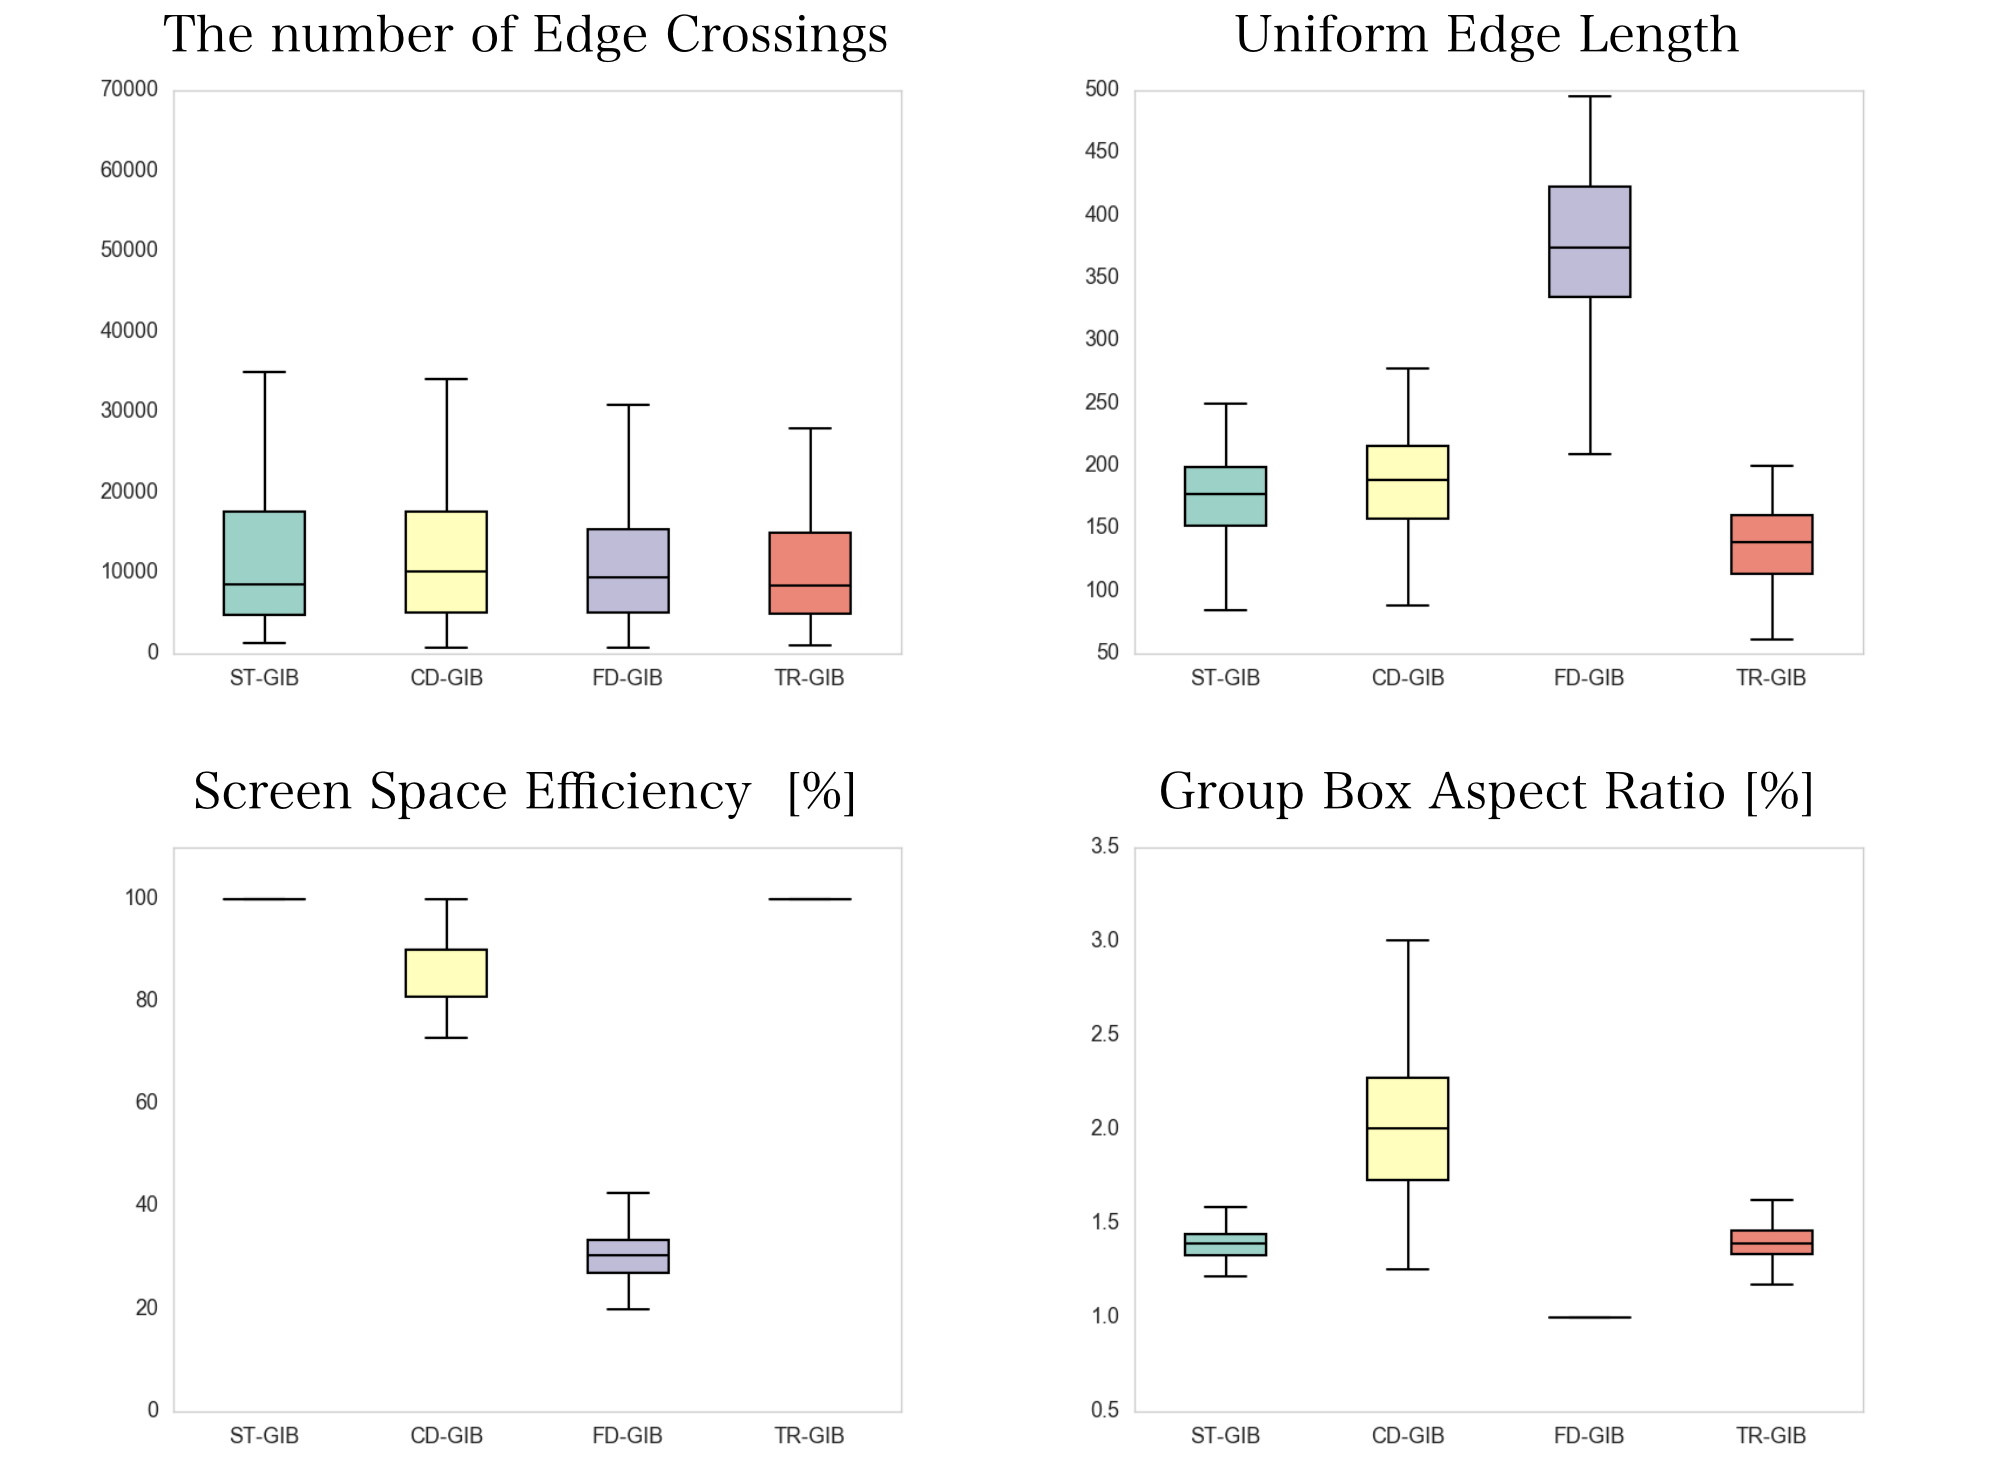
\includegraphics[width=0.5\textwidth]{pictures/computation.png}
    \caption{Computation results of the measures in graphs we used. We calculated 4 measures: the number of edge crossings, uniform edge lendth, screen space efficiency, and group box aspect ratio. These measures are known to affect the readability of a graph.}
    \label{comp-result}
  \end{center}
\end{figure}

Figure~\ref{comp-result} summarizes the calculation results.
In graph drawing, we demand fewer edge overlaps, smaller uniform edge length, lower aspect ratio and higher screen space efficiency.
The results show that TR-GIB had the fewest edge crossings and ST-GIB had the most, with the mean number of links of all graph is 541.2.
Considering TR-GIB achieved the best result and FD-GIB was the worst in uniform edge length, it is expected that participants would have a good result at user study in TR-GIB.


Regarding the screen space efficiency, it was low for ST-GIB and TR-GIB, followed by CD-GIB.
Furthermore, FD-GIB yielded the best aspect-ratio, followed by ST-GIB and TR-GIB.
ST-GIB and TR-GIB performed well in space efficiency and aspect ratio, whereas CD-GIB and FD-GIB performed well in terms of either space efficiency or aspect ratio.

As a summary, TR-GIB produced good results for all measures --- especially for edge crossing and uniform edge length.
CD-GIB and FD-GIB were poor in some measures, so we expect there are some trade-offs in the user study.
ST-GIB produced average results, except it had the most edge crossings, which could interrupt task performance.

%
\section{User Experiments}
%
In this study, we conducted user experiments with an eye-tracking system for various tasks to reveal which layout is superior.
The GIB layouts that we compared are ST-GIB, CD-GIB, FD-GIB, and TR-GIB.
In addition to the accuracy and completion time of tasks, we measured eye-tracking data to evaluate the layouts quantitatively.
This technique allows us to discuss our results in detail.


\subsection{Tasks}
\label{task}
We began the user study by setting up our tasks according to two previous studies: Vehlow et al.~\cite{Vehlow2017VisualizingGS} and Saket et al.~\cite{saket2014group}.
Vehlow et al.\ introduced four task taxonomies regarding the evaluation of clustered graph visualization, namely group-only tasks (GOTs), group vertex tasks (GVTs), group edge tasks (GETs), and group network tasks (GNTs).
Of these four tasks, we use GOTs, GVTs, and GNTs for our GIB evaluation; GETs are for networks whose edges are grouped, so we do not use this taxonomy.
Saket et al.\ provided four types of tasks, namely GOTs, group node tasks, group link tasks, and GNTs, all of which can be applied to ours, but we note that the GNTs used by Vehlow et al.\ is similar to the group link tasks used by Saket et al.
Vehlow et al.\ and Saket et al.\ also described examples of each task type: as a group node task, there is the task of finding the group with the most nodes.
We selected our tasks as follows.

\begin{itemize}
\item {\bf Task 1 (Group Only Task)}. How many groups are present in this graph?
\item {\bf Task 2 (Group-Node Task)}. Which group has the maximum (minimum) number of nodes?
\item {\bf Task 3 (Group-Intra-Link Task)}. Which group has the maximum (minimum) number of links?
\item {\bf Task 4 (Group-Inter-Link Task)}. Which group has the maximum number of links connecting its nodes outside the group?
\end{itemize}

Task 1 is a kind of GOTs from Vehlow's taxonomy and is about the number of groups represented. It requires no node or edge information but does require aggregate group information. We expect this task to determine which layout prompts understanding of the whole structure best.

Task 2 is from the GVTs and requires node information --- specifically the number of nodes. A GIB layout should be able to help users to estimate the size of a group easily, and this task can reveal which layout is the best in this respect.

Task 3 is a GNT, which requires intra-link information. An intra-link connects a node to another node in the same group, whereas a group inter-link connects a node to a node from another group.
In a layout with good representation of intra-links, users can easily understand the relationship within a group, which is often critical in the analysis process. We expect this task to derive the best layout for analysis within a group.

Task 4, another GNT, requires inter-link information.
An inter-link, showing a relationship between a couple of groups, sometimes becomes valuable and important information representing the coupling between clusters in a graph like a social network. We suppose that this task can detect a good layout for this purpose.

In Task 2 and Task 3, we set two tasks each, finding the maximum and the minimum number of nodes or links.
We suppose a GIB must be good at showing both large groups and small groups. In other words, a layout is not practical when it is good at showing only a group with many nodes (links) or few nodes (links).
We changed the task, namely maximum or minimum, at the half of total trials for Tasks 2 and 3.
We did not set two tasks in Task~4. This is mainly because we found it difficult to detect the group with the sparsest connections to other groups. A user experiment with low accuracy often involves random answers from users, which we aim to eliminate.

We elicit two tasks from GNTs, Task~3 and Task~4, because we aimed to assess the layout's capability of representing both group intra-links and group inter-links.
Because GIB is a method for visualizing the relationships among groups and within a group, the GIB layout method should be good at showing both of the intra- and inter-links.

\subsection{Hypotheses}
We constructed some hypotheses regarding our tasks.
From a previous work~\cite{chaturvedi2014group}, we know that there are differences among these four GIB variants, so we expect these layout variants to affect our tasks. It is noted that we focus on which elements cause differences in the results, for which we expect the eye-track analysis to help.

\begin{itemize}
\item {\bf Hypothesis 1}. Participants can complete Task~1 best with ST-GIB.
In ST-GIB, each box is organized in a row or a column, which makes it easier for the user to count more than one box at the same time.

\item {\bf Hypothesis 2}. In Task~2, ST-GIB achieves the best result.
In the algorithm we use, ST-GIB places boxes in order of their sizes. Therefore, the biggest / smallest box, the correct answer of Task~2, is always set at the left-top / right-bottom of the screen.
Participants should easily detect the answer.

\item {\bf Hypothesis 3}. In Task~2, CD-GIB is not as accurate as the others.
The box aspect ratio is poor with this layout, making it difficult to estimate the area at a glance.

\item {\bf Hypothesis 4}. In Task~3, TR-GIB gives the most accurate result.
This layout performs well in terms of aspect ratio and screen space efficiency as ST-GIB, so each network in a box can occupy more area than it can with CD-GIB or FD-GIB.
In addition, because we expect few edge crossings, we can see the intra-edges with fewer interruptions caused by inter-edges.

\item {\bf Hypothesis 5}. In Task~3, FD-GIB does not produce better results than the others because its boxes are smaller than those in other layouts.
If a box is small, the links in it are short, making it challenging to estimate the number of links visually.

\item {\bf Hypothesis 6}. In Task~4, TR-GIB and FD-GIB are more accurate than the other layouts.
TR-GIB is good at edge overlaps, making it easy to recognize the inter-links.
FD-GIB wastes space but provides areas for inter-links only, not boxes.
We expect it to be easy to observe inter-links with these two layouts.
\end{itemize}

\subsection{Experiment Design}

We used a repeated-measures study design, and the variables of interest were as follows.

\begin{itemize}
\item {\bf Layout of network diagram}. We used four GIB variants, namely ST-GIB, CD-GIB, FD-GIB, and TR-GIB.
\item {\bf Task}. We performed four tasks as described in Section~\ref{task}.
\end{itemize}

In terms of the amount of the experimental data, we generated 480 random networks in total; 120 were applied to each layout, and then they were allocated to the four tasks. Therefore, each task including stimuli of four layouts: 30 stimuli of the same layout in a task and in total 120.
A task had 6 sub-blocks with 20 stimuli so that participants could have small breaks among them.

Participants may have become confused if we changed the task for every trial, so the participants performed the same task continuously until the next break.
Additionally, the participants may have become accustomed to the data if we showed them network diagrams comprised of the same data, so we did not use any repeated data.

We randomized the stimuli order for each task, so the layout shown to participants changed at each trial.
We also randomized the task order to mitigate the effects of learning and fatigue.
Participants took a brief break of roughly 30~s after every 20 stimuli, a sub-block, and a relatively longer break after one task, 120 stimuli.
We empirically set the color as gray and the width of edges, as shown in Figure~\ref{GIB-examples}.

\subsection{Study Procedure}

The participants were asked to reveal their age, gender, and field of study in advance.
Next, they read a manual about biometric measuring, eye-tracking, and each GIB layout.
We then explained these experiments in detail, followed by a tutorial to check whether they could interpret the networks and solve our tasks.
The trial data of the tutorial differed from those in the actual experiments but nevertheless provided a practical guide to the experimental procedures.

Once the participants completed all the above steps, they proceeded to the actual experiments.
They worked on the four tasks in random order to compensate for the leaning and fatigue effects, and 120 trials existed in the same task.
For Tasks 2 and 3, we asked the participants two questions about the maximum or minimum: the first 60 trials asked for the maximum, and the last 60 trials asked for the minimum, where we permuted the trials so that each half had 15 networks for each layout in each task.

There was no time limit on the tasks, and the answers were sent to our server.
The participants were instructed to focus on answering correctly rather than the fast answer.
If they focused on answering quickly, we were likely to encounter higher error rates and more chaotic gaze trajectories, which was not the intention of this study.
The participants chose the solution by clicking and confirming it by pressing a button on a keyboard.

Figure~\ref{screenShot} shows a screenshot of the actual experiment (Task~2). Participants selected the biggest or smallest box and clicked on it. Participants could change their selection by clicking another box. When they pressed the Enter key, the answer and the completion time was sent to our server and then the next stimulus was shown.

\begin{figure}[t]
  \begin{center}
    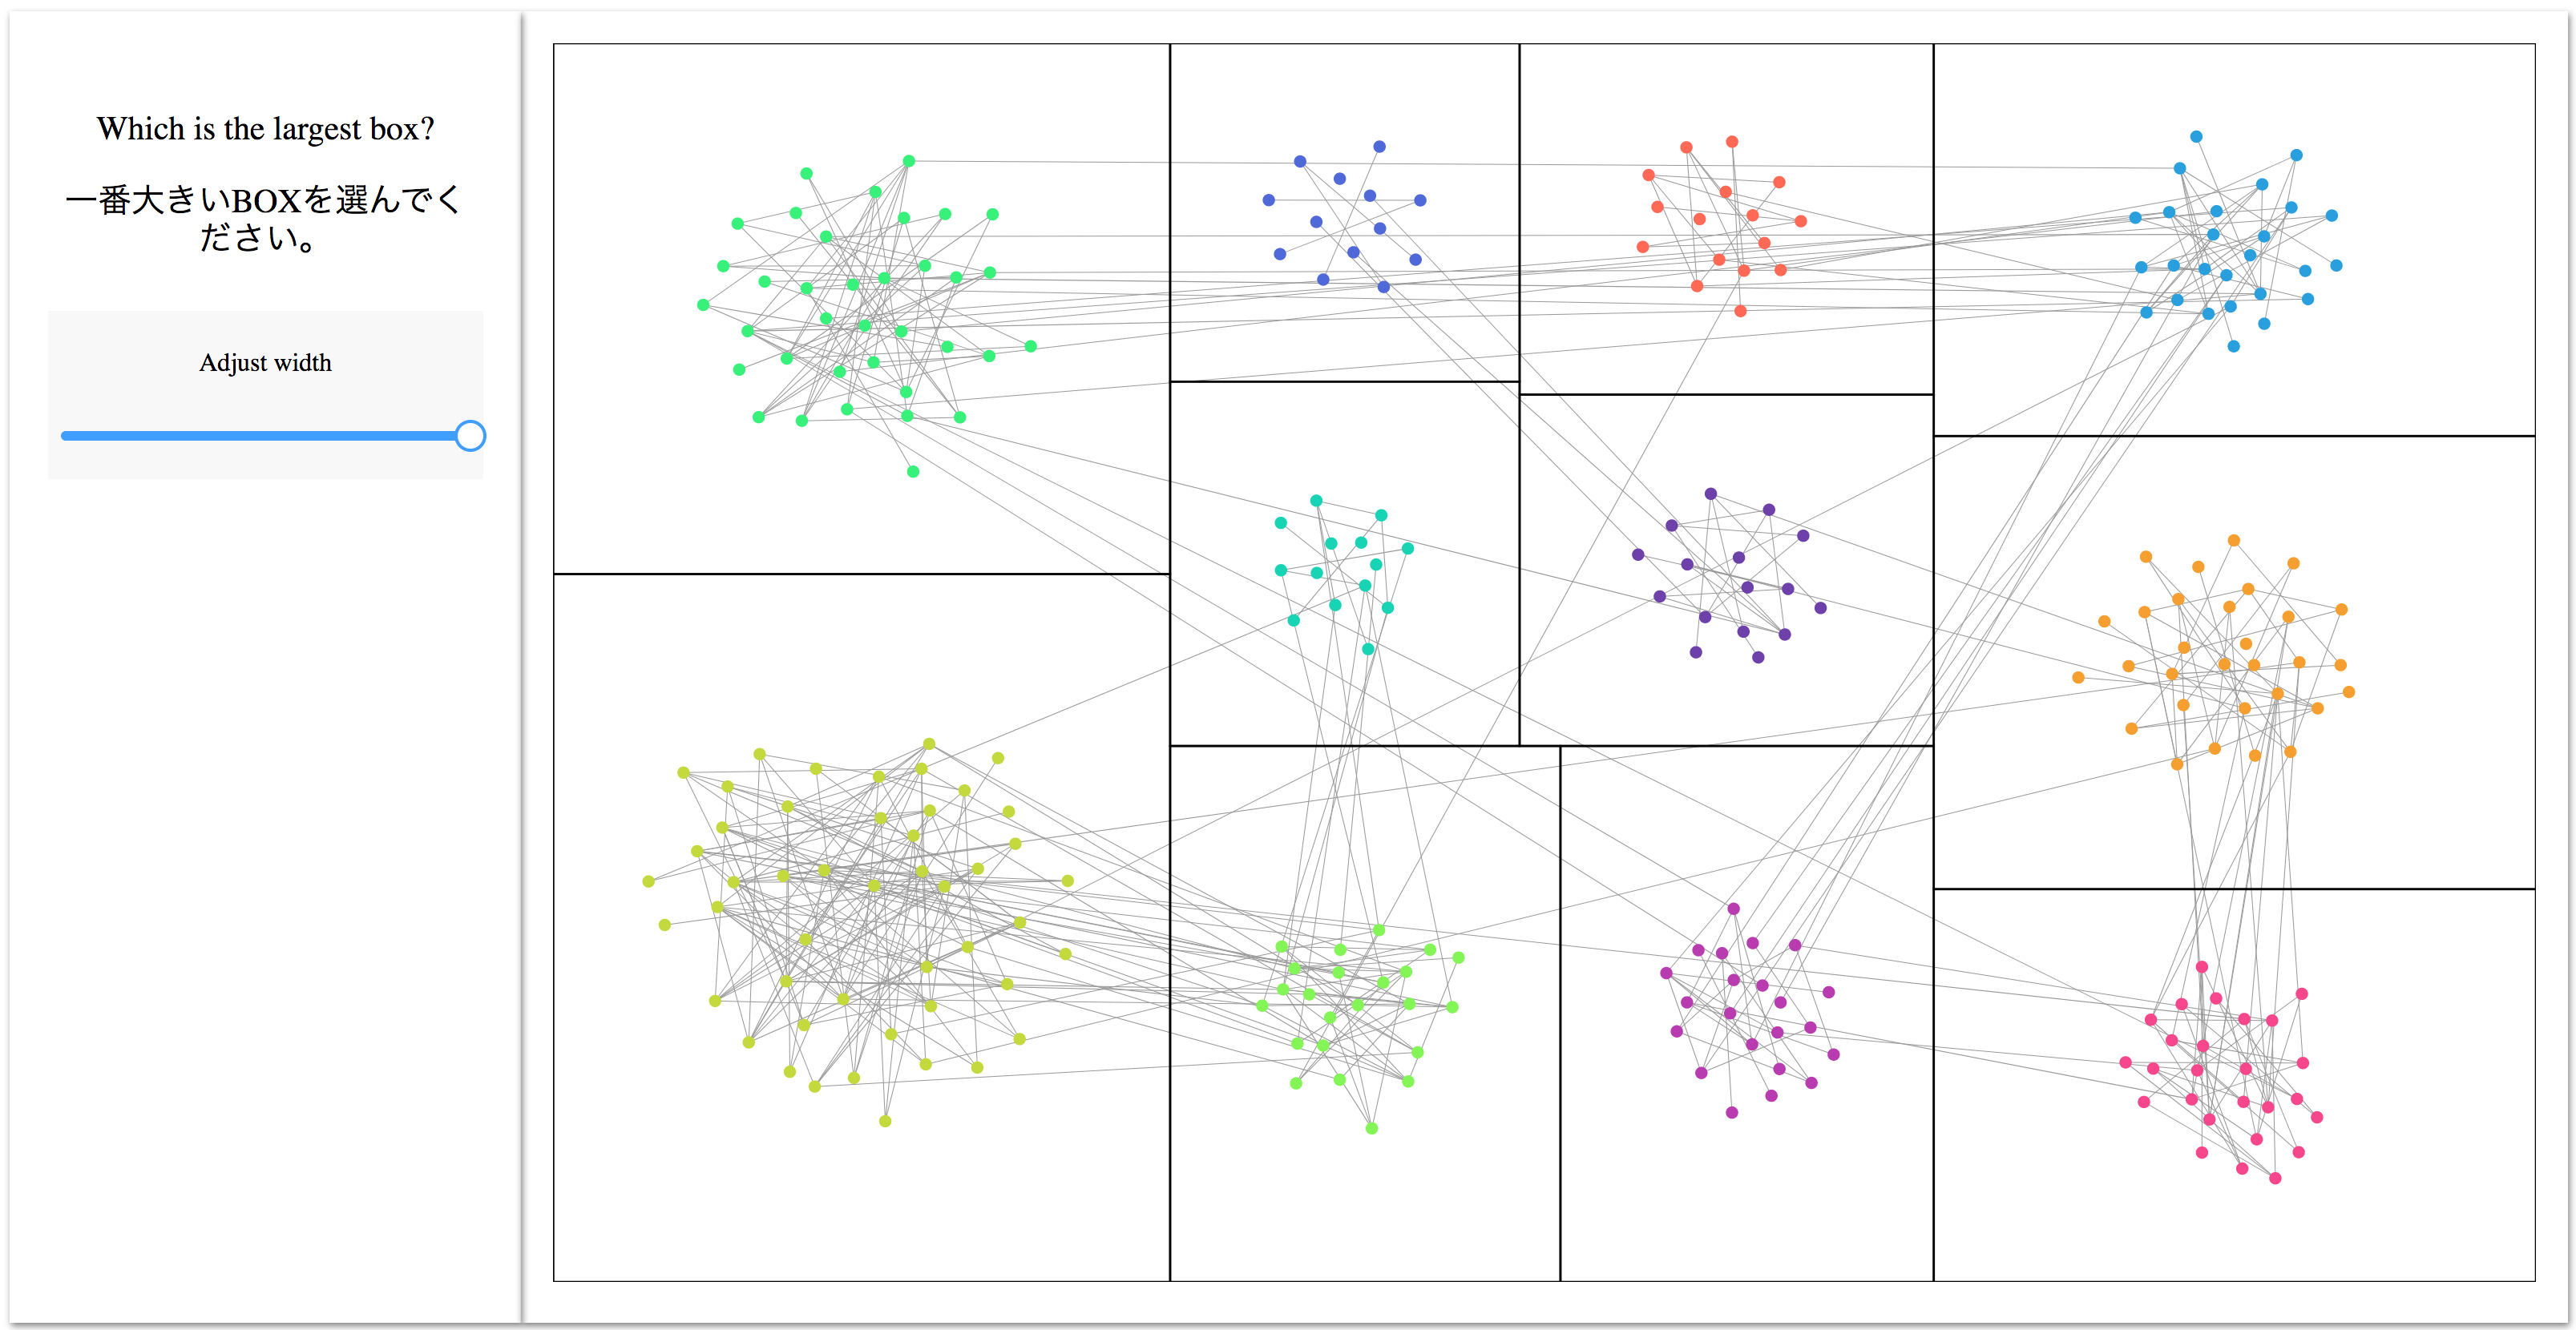
\includegraphics[width=0.45\textwidth]{pictures/screenshot.png}
    \caption{The actual experiment in Task 2, where the participants looked for the largest box.}
    \label{screenShot}
  \end{center}
\end{figure}

We conducted this eye-tracking experiment in a room with artificial illumination and a few objects.
The participants' mobile phones were switched off to reduce distractions during the experiments.
The eye movements were recorded using a Tobii Pro X3-120 eye-tracking system with an ASUS screen resolution of $2,018 \times 1,920$ pixels.
The participants sat in front of a display at a distance of 65~cm.
For the analysis software of the eye tracker, we utilized an I-VT filter to determine whether a gaze was a fixation or a saccade, as described in~\cite{olsen2012tobii}.

\subsection{Participants}

We used a within-subject study design with 20 participants, all of whom were Japanese (8 women and 12 men).
Their average age was 20.8 years, with the youngest participant being 18 and the oldest participant being 24.
All were students at our university: four were studying engineering, and the others had different majors.
All participants had normal or corrected-to-normal color vision.
Each participant was compensated with the sum of 3,000 Yen.
The experiment duration was 1.5--2 h, including the explanation and breaks.
We had a critical problem with the experiment system for 1 participant, so we excluded their data from the study, so we analyzed data from 19 participants in total.

\section{Experimental Results}

The goal of this study with eye tracking is to compare the readability of four layouts of GIB with some tasks. We collected the task correctness and completion time as well as the gaze data during the user experiments.
From here, we describe the result of the experiments divided into two parts: the correctness and the completion time in Section~\ref{taskResult}; eye-track data based on our hypotheses in Section~\ref{eyetrack}.

\subsection{Task Results}
\label{taskResult}

In this subsection, we describe the results of the user experiments, excluding the eye-tracking data, which are discussed in the following subsection.
This subsection presents the results of the statistical analysis of completion time and correctness of all tasks.
As the data were not normally distributed, we used non-parametric analysis methods for the analysis.
We conducted the Friedman test to determine whether there was a significant difference, followed by the post-hoc Wilcoxon signed rank test. In all cases, we used $0.05$ as a significance value.
Hereafter, the statistical analyses are discussed for each task separately, where we supposed that each layout has its advantages and disadvantages and that all tasks are independent.

\begin{figure*}[t]
  \begin{center}
    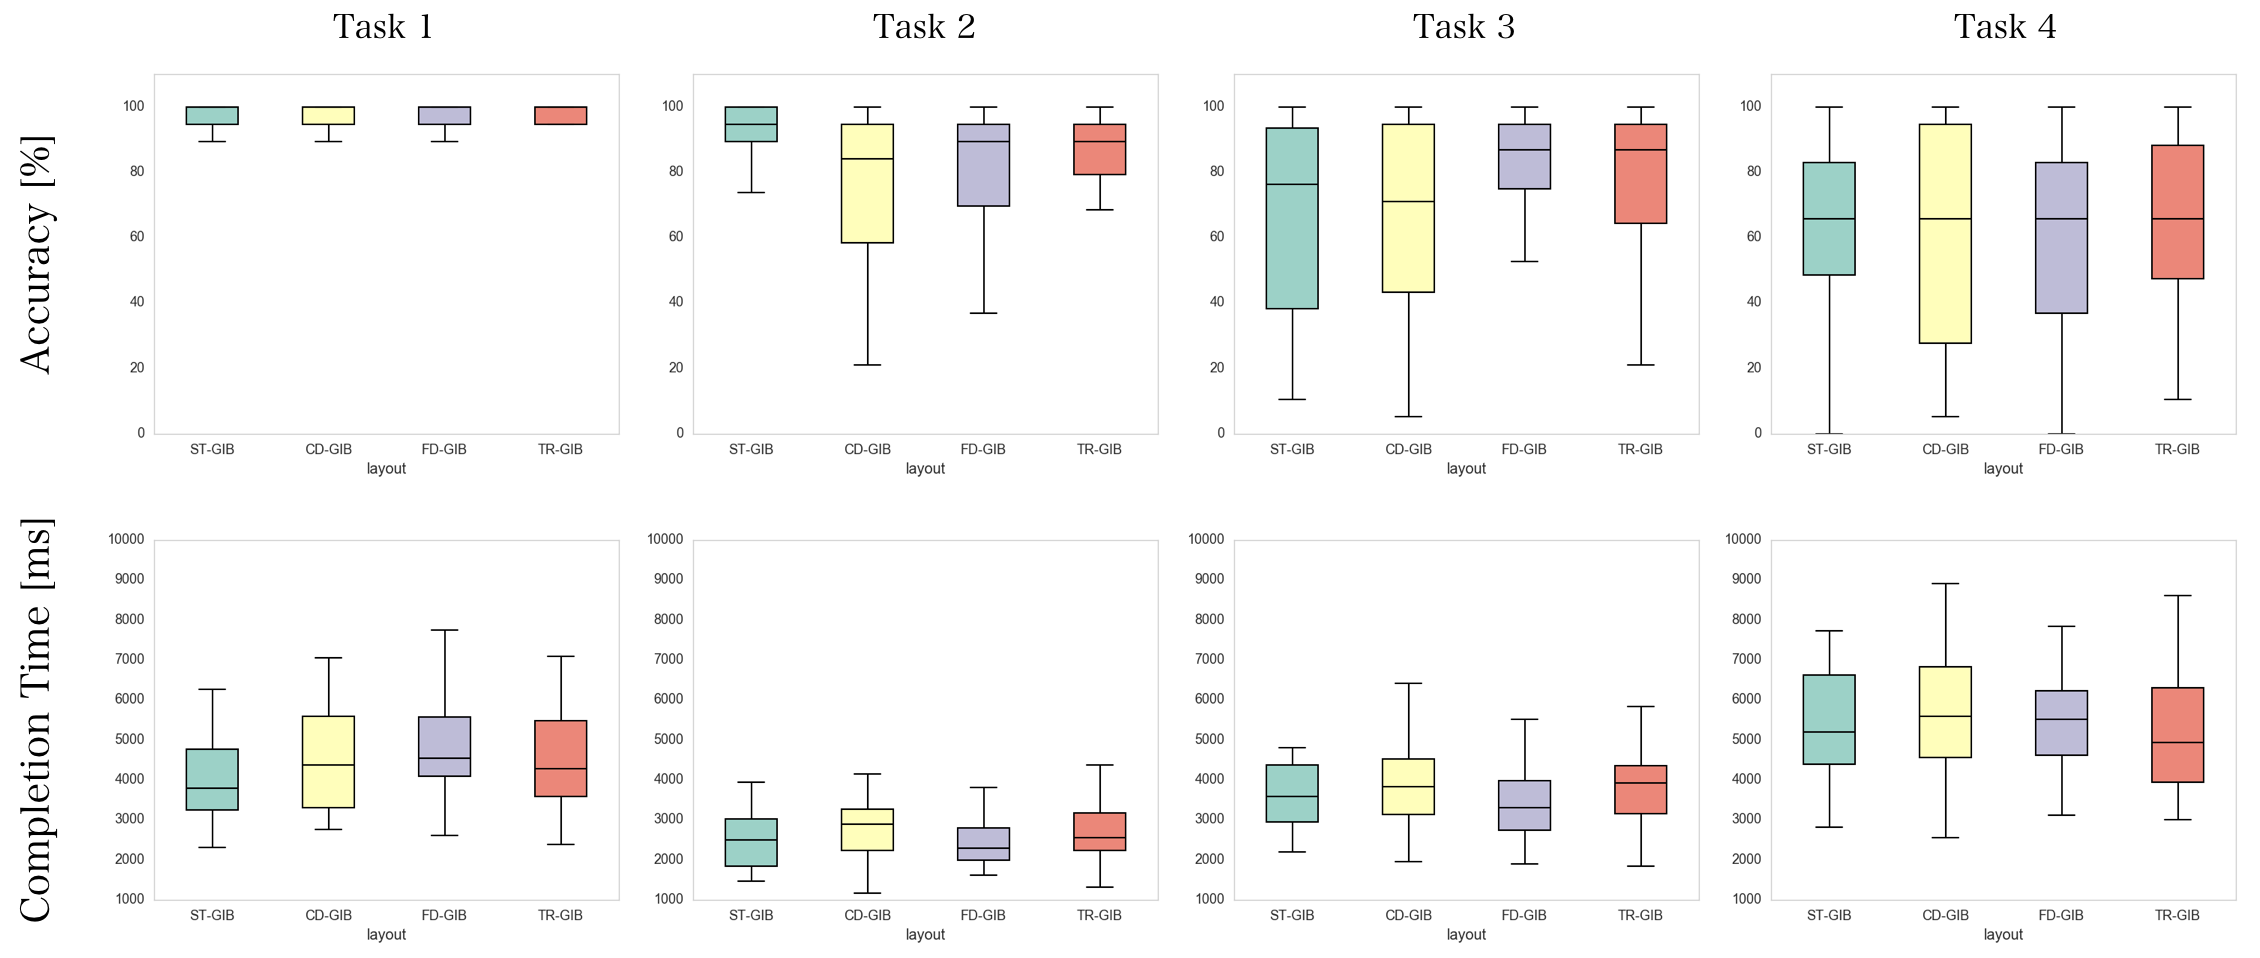
\includegraphics[width=1\textwidth]{pictures/results.png}
    \caption{The result of the task. The upper row represents the accuracy at each task, and the lower is for the completion time. The column shows the variation of tasks. For example, the box graph on the upper row and the second from the left show the accuracy in Task 2.}
    \label{results}
  \end{center}
\end{figure*}

% \begin{table}[htb]
%   \begin{center}
%     \begin{tabular}{|c||c|c|c|c|} \hline
%       Layout & Task 1 & Task 2 & Task 3 & Task 4 \\ \hline \hline
%       ST-GIB & 98.1\% (3.987~s) & 89.6\% (2.535~s) & 67.4\% (3.606~s) & 62.8\% (5.387~s) \\ \hline
%       CD-GIB & 98.2\% (4.527~s) & 76.9\% (2.761~s) & 67.2\% (3.843~s) & 59.3\% (5.588~s)\\ \hline
%       FD-GIB & 96.7\% (4.919~s) & 82.9\% (2.427~s) & 78.8\% (3.382~s) & 59.3\% (5.518~s)\\ \hline
%       TR-GIB & 98.1\% (4.493~s) & 83.6\% (2.713~s) & 72.8\% (3.845~s) & 63.5\% (5.128~s)\\ \hline
%     \end{tabular}
%   \end{center}
%    \caption{Results of user study: mean accuracy (mean completion time)}
%   \label{user-result}
% \end{table}

{\bf Task 1.} The mean accuracy of all layouts was 97.7\% and the mean completion time was 4480 ms.
Figure~\ref{results} shows the accuracies and completion times of the 4 tasks. Friedman analysis gave a significant effect in completion time ($p < 0.001$) while no significant difference in the correctness was found.
The post-hoc Wilcoxon test found that participants completed this task significantly earlier in ST-GIB and TR-GIB than in CD-GIB and FD-GIB ($p<0.001$), and also CD-GIB is faster than FD-GIB ($p<0.001$).

The time required for ST-GIB in this task was approximately 500 ms shorter than that of CD-GIB and TR-GIB, and 900 ms shorter than that of FD-GIB on average.
These results support Hypothesis~1.

{\bf Task 2.} ST-GIB was the best in terms of accuracy with a mean accuracy of 89.6\% and completion time of 2526 ms, and FD-GIB had the fastest completion time with a mean accuracy of 83.0 \% and completion time of 2425 ms.
Friedman test presented significant differences in both correctness ($p<0.001$) and completion time ($p = 0.0025$) for this task.
The Wilcoxon test showed significant effectiveness of ST-GIB compared to all other layouts ($p<0.001$ for CD-GIB and FD-GIB; $p=0.0019$ for TR-GIB), and ineffectiveness of CD-GIB compared to all others ($p<0.001$ for ST-GIB; $p=0.0041$ for FD-GIB; $p=0.0019$ for TR-GIB).

These results support Hypothesis~2 and Hypothesis~3. FD-GIB and TR-GIB were better than CD-GIB, but not as effective as ST-GIB, which places boxes in order of their sizes.

{\bf Task 3.} FD-GIB had the highest scores for both accuracy (78.8\%) and time (3383ms).
The Friedman test shows that there were significant differences in both correctness and completion time ($p<0.001$).
According to the Wilcoxon test, FD-GIB was better than all other layouts in terms of correctness ($p<0.001$ for ST-GIB and CD-GIB; $p=0.017$ for TR-GIB) and completion time ($p=0.007$ for ST-GIB; $p<0.001$ for CD-GIB and TR-GIB). It also shows significant differences in correctness for TR-GIB over ST-GIB ($p=0.039$) and CD-GIB ($p=0.049$), and participants finished Task 3 earlier in ST-GIB than CD-GIB ($p=0.014$) and TR-GIB ($p=0.014$).

These results contradict Hypothesis~4 and Hypothesis~5: FD-GIB performed this task with the best accuracy and completion time. TR-GIB did not produce bad results, but its accuracy was $6 \%$ lower and it required 500 ms longer to complete this task than FD-GIB.

{\bf Task 4.} The mean accuracy of all layouts was 61.2\% and the mean completion time was 5405 ms.
The Friedman test shows there was a significant difference in completion time ($p = 0.039$).
The Wilcoxon test shows that participants reached their answers 400 ms earlier in TR-GIB than in FD-GIB ($p=0.003$).



% \begin{table}[h]
%   \begin{center}
%     \begin{tabular}{|c||c|c|c|c|} \hline
%       & Task 1 & Task 2 & Task 3 & Task 4 \\ \hline \hline
%         Accuracy & 0.2377 & 2.579e$-7$ & 1.303e$-5$ & 0.3039 \\ \hline
%         Time & 9.009e$-16$ & 7.571e$-5$ & 4.706e$-5$ & 0.06275\\ \hline
%     \end{tabular}
%   \end{center}
%   \caption{P-values of ANOVA for accuracy and completion time}
%   \label{anova}
% \end{table}

\subsection{Eye-tracking Results}
\label{eyetrack}
In this section, we present the results of eye tracking during the experiments and compare the collected data with our hypotheses.
There are many methods in eye-track analysis, and they are mainly divided into two categories. One is the use of some computation measures, such as fixation duration or saccade length.
These measures allow researchers to conduct statistical analyses because of their quantitative nature.
In this study, we often used the number of distractors before or after a participant gazed at the correct answer for the first time as a measure.
A distractor is a box other than the correct answer.
Hereafter, we call this measure before the first gaze at the correct answer {\bf DB} and of the measure after the first gaze {\bf DA}.

Another method is visual analytics with some visualizations for eye-track data such as trajectory map, gaze heat map, or flow map.
There are also several studies providing guidelines on the analysis of eye tracking data~\cite{andrienko2012visual,duchowski2007eye,kurzhals2014evaluating}. In order to analyze our data, we aim to use these various methods. We would like to emphasize that the main purpose we use eye tracking for in this study is finding which elements in a GIB layout help or interrupt task performance. Therefore, in this section, we describe our eye-tracking analysis based on our hypotheses considering visual attributes in GIB.

{\bf Hypothesis~1.} This hypothesis can be confirmed by our experiment where ST-GIB achieved the highest accuracy.
To verify our hypothesis, we computed an eye-track measure --- gaze count.
The result is shown in Table.~\ref{gazecount}.
We conducted a statistical analysis using the Friedman test as described in Section~\ref{taskResult}.
We found a significant difference in the gaze counts for the four GIB layouts ($p=0.040$). A post-hoc Wilcoxon test shows that ST-GIB did not have as many gaze counts as the others, where $p<0.001$. Fewer gaze counts indicate that there were few recounting or some multiple counts at the same time, where participants might easily count the number of groups. Therefore, this eye track measure supports this hypothesis and we suppose the well-aligned boxes can help with the counting.

\begin{table}[b]
  \begin{center}
    \caption{Mean gaze counts (standard deviation)}
    \label{gazecount}
    \begin{tabular}{|c|c|c|c|c|} \hline
      & ST-GIB & CD-GIB & FD-GIB & TR-GIB \\ \hline
      Task~1 & 12.5 (5.49) & 14.4 (6.79) & 15.6 (6.85) & 14.1 (6.31) \\ \hline
      Task~2 & 8.6 (5.11) & 9.2 (5.30) & 8.3 (4.04) & 9.1 (5.18) \\ \hline
    \end{tabular}
    \end{center}
\end{table}

{\bf Hypothesis~2.} ST-GIB achieved the best result for Task 2, which supports this hypothesis. As shown in Table.~\ref{gazecount}, ST-GIB and FD-GIB did not require as many gazes as CD-GIB and TR-GIB. From the Friedman test, there were significant differences in the number of gazes between ST-GIB and CD-GIB ($p=0.002$), between FD-GIB and CD-GIB ($p=0.002$), and between FD-GIB and TR-GIB ($p<0.001$). Another measure, {\bf DB} shows evidence of this hypothesis and is shown in Table~\ref{table-dist2}. We observed a significant difference in this measure ($p=0.009$), and this in ST-GIB was significantly lower than in CD-GIB ($p=0.027$) and FD-GIB ($p=0.006$). This indicates that participants could easily reach the correct answer in ST-GIB, and we suppose this happened due to the boxes being sorted by size.

{\bf Hypothesis 3.} This hypothesis is supported by the results of Task~2 where CD-GIB was the worst for the correctness. In CD-GIB, it is inferred that some visual attributes prevented the participants from guessing the area visually.
We supposed that this is due to the poor aspect ratio of boxes, which might have confused participants. We also found a clue to reveal which element in this layout interrupted the task performance in a gaze flow map shown in Figure~\ref{task2flow}.
A gaze flow map represents the flow of fixation of all participants among boxes, and the width of each flow is proportional to the number of transitions of gaze from one box to another. We only visualize flows with transitions representing more than 3 \% of the whole. In the CD-GIB, candidate boxes for area comparison are sometimes placed apart, so the area comparison might be difficult.
Although TR-GIB had many gaze counts for CD-GIB, boxes that are candidates for area comparison are often located nearby since TR-GIB is what we reordered the tiles in ST-GIB with keeping the structure of a treemap, which shows that comparative work is relatively easy.

This figure also shows the difficulty of area comparison of boxes with poor aspect ratio: one of the three comparison targets is the horizontally longitudinal rectangle, which is not easy to estimate in size visually. Therefore, we suppose the poor aspect ratio and the fact that boxes with close areas were placed apart resulted in low accuracy.

\begin{figure}[t]
  \begin{center}
    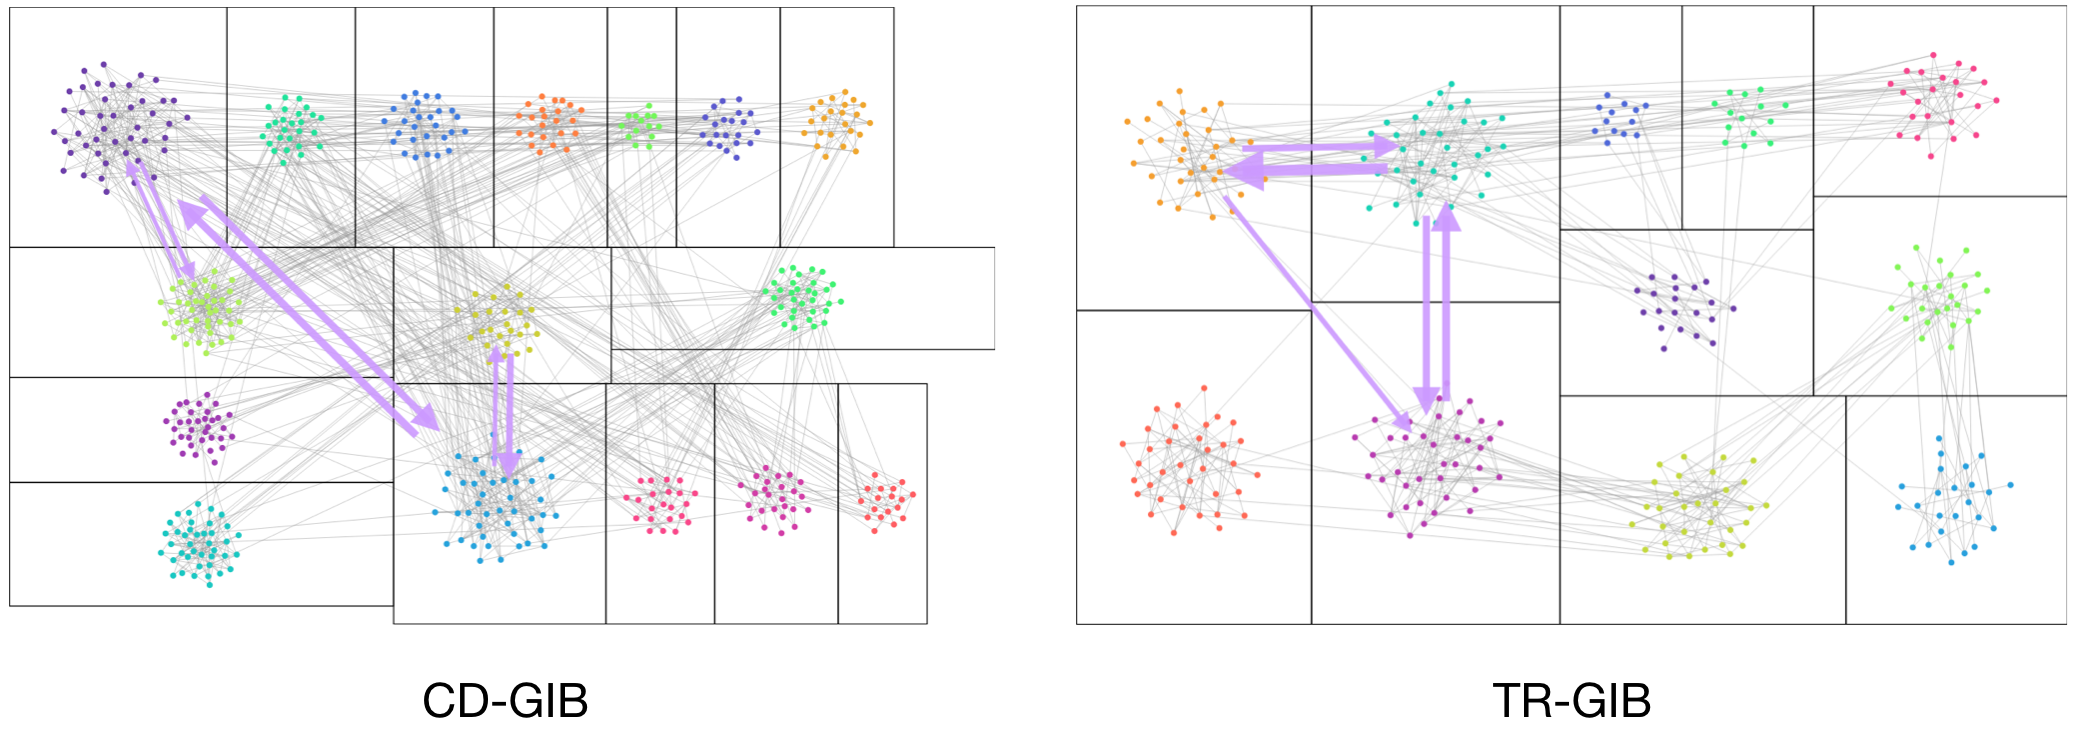
\includegraphics[width=0.48\textwidth]{pictures/cd-tr-in2.png}
    \caption{Flow map of CD-GIB and TR-GIB in Task~2. The boxes gazed were the candidate for the comparison to detect the answer, which were placed aprt in CD-GIB and nearby in TR-GIB.}
    \label{task2flow}
  \end{center}
\end{figure}

{\bf Hypothesis 4.} TR-GIB did not produce the best result in Task~3 and this hypothesis could not be confirmed, although this layout resulted in significantly higher correctness than ST-GIB and CD-GIB.
We suppose that the superiority of this layout lies in the small number of edge crossings and because intra-links are presented more clearly when there are fewer interferences by inter-links.
Table~\ref{table-dist3} also gave us a clue about this result.
TR-GIB and ST-GIB had the smallest numbers of {\bf DB}.
We observed a significant difference in this measure by Friedman test, where $p<0.001$, and those of TR-GIB and ST-GIB are significantly smaller than those of CD-GIB and FD-GIB ($p<0.001$) in the Wilcoxon post-hoc test.
This means that participants did not require as many gazes to reach the correct box in TR-GIB and ST-GIB compared to CD-GIB and FD-GIB.
The boxes in TR-GIB and ST-GIB are well-arranged horizontally or vertically.
We suppose this aligned arrangement helped the participants to find the correct answer in Task~3 as well as in Task~2.
The task to find the box with the biggest / smallest number of intra-links tended to depend on detecting the box with the biggest / smallest area because a big box often had many intra-links in both our algorithm and the real-world network.

Although ST-GIB was good at {\bf DB} above, it did not achieve high accuracy.
It was easy to gaze at the correct answer as a candidate in Task~3 because of the well-aligned boxes, but the higher number of edge-crossings might have made it challenging to compare the numbers of intra-edges.


{\bf Hypothesis 5}. Since FD-GIB achieved the best result in Task~3 in spite of its small boxes, this hypothesis was refuted. In FD-GIB there are not as many edge crossings as in ST-GIB and CD-GIB, so it might have been easier to see the intra-links here. Therefore, this result means the number of edge crossings should have been small, but the box size did not have to be large in this task.
Table~\ref{table-dist3} showed that the participants required a large number of gaze counts before the first gaze at the correct answer, but the number of gaze points to the distractor after that was the smallest; we observed a significant difference ($p<0.001$) in {\bf DA} and post-hoc analysis showed that {\bf DA} in FD-GIB is significantly smaller than for the others ($p<0.001$ for ST-GIB and TR-GIB; $p=0.001$ for CD-GIB).
This result indicates that the participants took many gazes before gazing at the correct answer even as a candidate, but it required only a little thought to make their decisions after the first gaze.
We suppose this is because the participants estimate the number of intra-links visually ambiguously, and specifically they saw the links as a color.
Since we draw the edges with gray color, the number of edges could be seen as the density of the color representing the degree of aggregation.
Moreover, a box in FD-GIB is much smaller than for the others, so this trend might be particularly remarkable since the degree of aggregation become greater.
% Therefore, we can say that FD-GIB would be effective to understand the abstract information about intra-relationships such as the number of intra-links, but for more concrete information another layout would be more effective such as TR-GIB.

\begin{table}[b]
  \begin{center}
   \caption{Gaze count of distractors in Task~2 (standard deviation)}
  \label{table-dist2}
    \begin{tabular}{|c|c|c|c|c|} \hline
      & ST-GIB & CD-GIB & FD-GIB & TR-GIB \\ \hline
      % Task 1 & 12.5 (5.49) & 14.4 (6.79) & 15.6 (6.85) & 14.1 (6.31) \\ \hline
      {\bf DB} & 3.6 (3.59) & 3.9 (3.67) & 4.1 (3.48) & 3.7 (3.06) \\ \hline
      {\bf DA}  & 2.84 (3.33) & 2.99 (3.67) & 4.1 (3.48) & 3.7 (3.06) \\ \hline
    \end{tabular}
  \end{center}
  \begin{center}
   \caption{Gaze count of distractors in Task~3 (standard deviation)}
  \label{table-dist3}
    \begin{tabular}{|c|c|c|c|c|} \hline
      & ST-GIB & CD-GIB & FD-GIB & TR-GIB \\ \hline
      % Task 1 & 12.5 (5.49) & 14.4 (6.79) & 15.6 (6.85) & 14.1 (6.31) \\ \hline
      {\bf DB} & 3.8 (4.64) & 5.1 (5.11) & 4.8 (4.38) & 3.8 (4.48) \\ \hline
      {\bf DA} & 4.8 (4.65) & 4.8 (4.84) & 3.7 (4.27) & 5.3 (5.37) \\ \hline
    \end{tabular}
  \end{center}
\end{table}


\begin{figure}[t]
  \begin{center}
    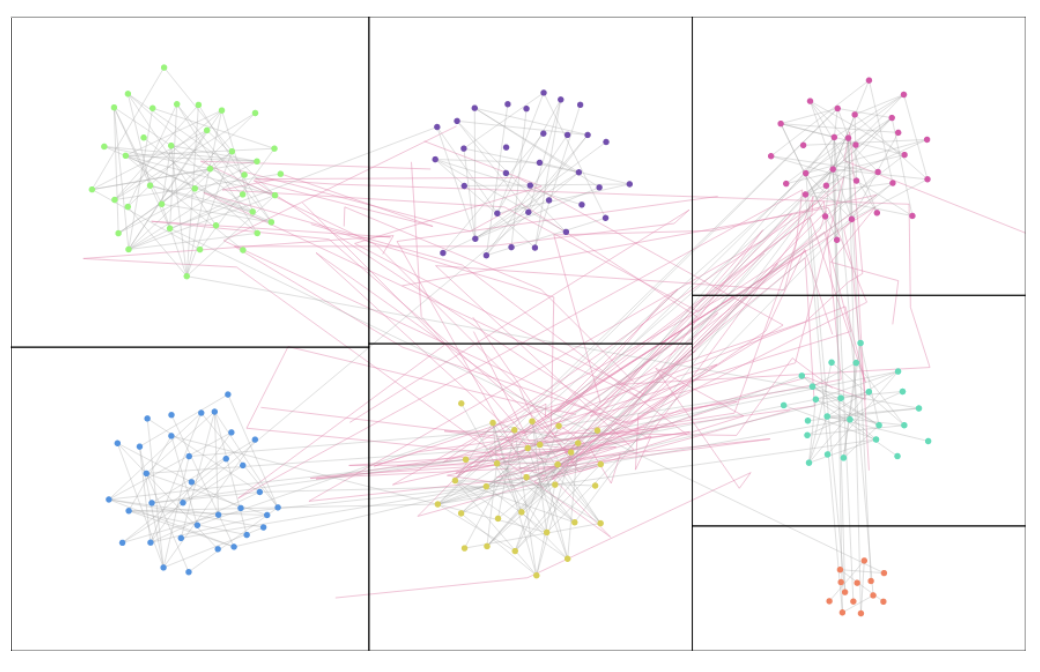
\includegraphics[width=0.33\textwidth]{pictures/concentration.png}
    \caption{Trajectory map for Task~4. The gaze movement is represented with a pink line and there is a gaze aggregation on a bundle of inter-links.}
    \label{concent}
  \end{center}
\end{figure}

{\bf Hypothesis 6}. We found no significant difference in the correctness of Task~4, and this hypothesis could not be confirmed.
The four layouts have differences in their edge crossings and uniform edge lengths, which are thought to affect the readability of a graph -- especially link information -- but they did not make any difference.
We observed that the completion time of TR-GIB was statistically shorter than that of FD-GIB.

Regarding the computation result in Figure~\ref{comp-result}, we expected there would be a difference in the correctness as we observe differences in the number of edge crossings and uniform edge length.
As a reason for this task's result, we found a gaze concentration in a trajectory map of this Task~as shown in Figure~\ref{concent}.
The gaze data (pink line) are concentrated so as to overlap the bundle of inter-links, and we found this trend in many cases in this task.
Therefore, we suppose that the participants were searching for the answer with this bundle as a clue.
Since certain group pairs in our graph have some strong connections, there were some link bundles of straight lines.
Moreover, when we search for a link bundle, a longer bundle which is undesirable for graph drawing often stands out visually more than a shorter one.
The long bundle of inter-links might have affected the result in this task, resulting in no difference in the correctness. 

\section{Discussion}
We describe the further discussion in this section, not only based on eye-track data. From here, we describe the experimental results for the four tasks.

{\bf Task~1}. This task was very simple with just counting the number of the boxes, but the four layouts made a statistical difference in the result at completion time.
Eye-track analysis gave us a clue that the well-aligned ST-GIB was effective in this task.
We also found that FD-GIB required the longest duration to detect the answer, where each box was smaller than the other layouts and was placed apart.
With respect to Hypothesis~1, boxes should be well-arranged horizontally or vertically and presented with large size to count the number of them.

{\bf Task 2}. In this task, ST-GIB achieved the best accuracy, where boxes were placed in order of area, and the aspect ratio of a box was not poor.
CD-GIB with bad aspect ratio of boxes was not as accurate as the other layouts, while FD-GIB with the best aspect ratio was accurate and the fastest.
Therefore, a layout with good aspect ratio might be effective to detect the largest or smallest box.
We also reveal that the distance between the boxes as the candidates for comparison of the size is important.
Figure.~\ref{task2flow} shows that the boxes with similar size can be placed apart.
When these boxes which are the candidates for the comparison are placed next to each other as in ST-GIB and TR-GIB, the comparison process would be easier.

{\bf Task 3}. Participants were required to detect a box with the most or fewest intra-links.
For Hypothesis~4, we assumed that the number of edge crossings was important in this task, which indicates that it was challenging to discriminate an intra-link from an inter-link.
As a result, TR-GIB and FD-GIB, which are the layouts with fewer edge crossings, had higher accuracies than the others.
Computational measures of eye tracking, namely {\bf DB} and {\bf DA}, gave us evidence of this result.
TR-GIB had well-aligned boxes and the smallest {\bf DB}, which indicates that the ease of comparison of box sizes made it easier to reach the correct answer, and the fewest number of edge crossings and the best uniform edge length helped to decide the answer correctly.

FD-GIB had the highest correctness and the smallest {\bf DA}.
This indicates that the small box in FD-GIB was enough to complete this task and it also encouraged the performance.
The smallest {\bf DA} also mean that the shortest comparison process after the first gaze on the correct answer.
With respect to the small boxes in FD-GIB, in addition to this result, we suppose that participants could solve this task only by seeing the color of a box, which represents the density of links.
We set this task to reveal which layout is the best for representing intra-links.
From the studies of the survey about graph drawing for group structure~\cite{Vehlow2017VisualizingGS,saket2014group}, there is another task suitable for this purpose --- finding the vertex with the highest degree in a particular group.
This task requires more concrete information than we collected, and FD-GIB might be not appropriate for this task because of its small boxes and poor uniform edge length.
We revealed the effectiveness of FD-GIB and TR-GIB in this task, but some computation measure showed the difference between them so another task will be interesting.


{\bf Task 4}. We did not find any difference in the result of correctness, and TR-GIB did not require as much time to complete this task as FD-GIB.
Various factors can be considered as a cause of this, but in this study, we were unable to find a difference with respect to the visibility of inter-links.

{\bf Summary}. We found some trade-offs among each method for the type of user task.
ST-GIB achieved the best results in Task~1 and Task~2, while CD-GIB did not achieve a remarkable result.
FD-GIB was not poor in all tasks, and it had the best result in Task~3.
Participants also achieved averages scores in all tasks in TR-GIB.

In the actual analysis of real-world data, a graph must display links comprehensively.
In Task~3, FD-GIB and TR-GIB achieved good results and were average in other tasks, so we conclude that these two layouts are superior.
Since we found some trade-offs in the task results, we recommend selecting one based on the user's purpose.
If a user wishes to know the aggregate and abstract information of the graph, we suppose that FD-GIB is the best.
Participants completed Task~2 and Task~3 fastest in FD-GIB where a box is represented as smaller, so this layout is suited for quick and uncomplicated tasks.
On the other hand, TR-GIB can display the link information more concretely because of its good space efficiency.
This layout did not result in bad scores in any tasks, so it may be of help to users to see the relationships of nodes clearly because of the result of Task~3.


\section{Website for the GIB layouts}
As part of our work, we provide a website that enables anyone to access the four GIB layouts easily~\cite{gibweb}.
Users can easily get the GIB layouts in the form of a bitmap or svg image file with their own data.
This enables further analysis.
Figure~\ref{website} shows a screenshot of the website.
There, you can select any node by click, and then the node will be highlighted as well as the links connected to it.
You can see detailed information on the node by hovering the mouse over it.
We hope this work can aid many researchers by providing many GIBs.

\begin{figure}
  \begin{center}
    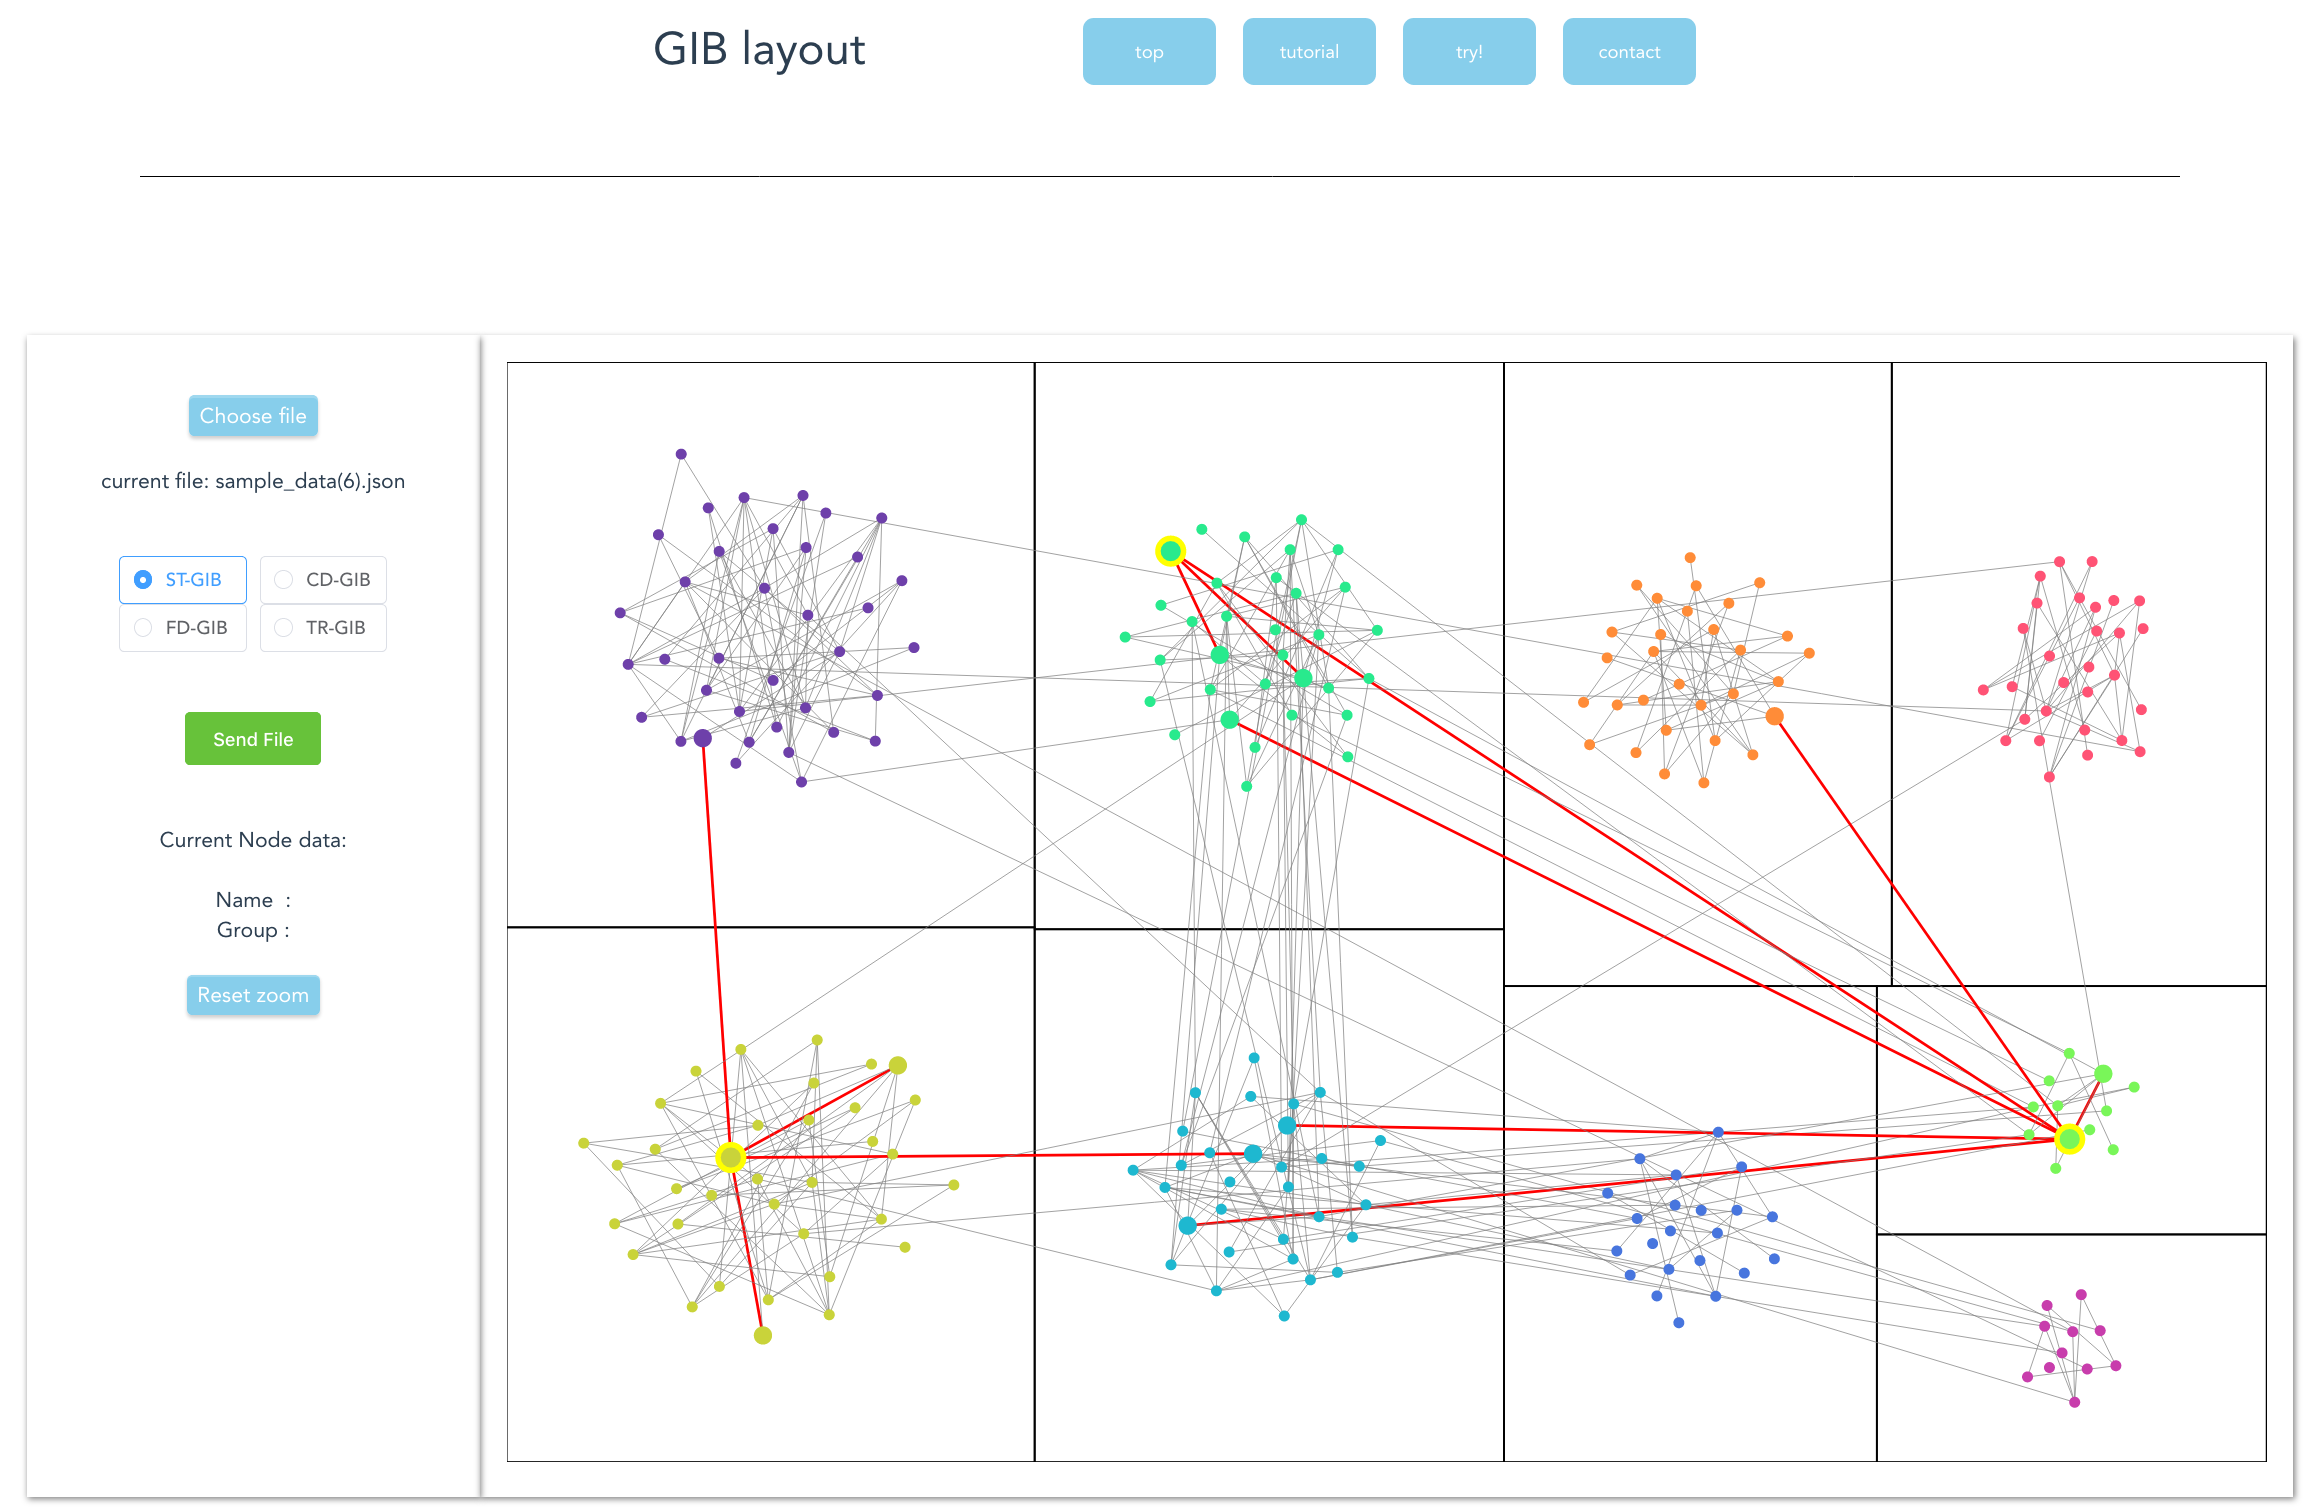
\includegraphics[width=0.48\textwidth]{pictures/website.png}
    \caption{The website we constructed. This site make it possible to get the four GIB layouts to the public, and it also provides further interactive analysis.}
    \label{website}
  \end{center}
\end{figure}

%
\section{Conclusion}
%

In this study, we evaluated four GIB layouts by means of a user study with eye tracking.
We determined which layout is the best with four tasks and obtained evidence to support the results with eye tracking.
The best layouts were FD-GIB and TR-GIB, which achieved higher performances, with both layouts having their own advantages and disadvantages.
FD-GIB performed well in determining the number of links, a blurred information, whereas TR-GIB would be better in representing more concrete relationships, e.g., links between two specific nodes.
ST-GIB performed well in terms of understanding the size of each box; however, it was poor in interpreting links.

Eye-track data gave us evidence of the result and interesting clues to reveal which elements in a visualization affect task performance.
For example, the well-aligned ST-GIB helped to count the number of groups.
We also found that the candidates for comparison were often placed apart in CD-GIB, which caused poor task performance.
Furthermore, the poor screen space efficiency in FD-GIB helped to estimate the number of intra-links, resulting in the fewest gaze counts after the first gaze at the correct answer.

We also provide a website where anyone can access the four GIB layouts easily.
We hope this work can contribute to meaningful discoveries by many researchers.

Regarding the limitations of this work, other algorithms or methods could be used to generate random data, although we aimed to make them realistic.
In particular, we used only one set of parameters in the user study; thus, other cases would be of interest.
Additionally, there are several other ways to express nodes and edges and arranging nodes, which may influence the results.
We found that undesirable long edges were effective in Task~4; therefore, another task may lead us to further results.

Our massive eye-tracking data could be used for further analysis as a future work.
Many other methods are available for dealing with eye-tracking data, which may lead to novel discoveries.

% \section{Acknowledgments}
% This work was supported by JST CREST Grant Number JPMJCR1511, Japan.


%\bibliographystyle{abbrv}
\bibliographystyle{abbrv-doi}
%\bibliographystyle{abbrv-doi-narrow}
%\bibliographystyle{abbrv-doi-hyperref}
%\bibliographystyle{abbrv-doi-hyperref-narrow}

\bibliography{template}
\end{document}
